\documentclass[12pt, letterpaper]{scrartcl}
\usepackage[utf8]{inputenc}
\usepackage{graphicx}
\usepackage{fancyhdr}
\usepackage{hyperref}
\usepackage{subfig}
\usepackage{float}

\usepackage{scalerel,amssymb}

\newcommand\equalhat{%
	\let\savearraystretch\arraystretch
	\renewcommand\arraystretch{0.3}
	\begin{array}{c}
		\stretchto{
			\scalerel*[\widthof{=}]{\wedge}
			{\rule{1ex}{3ex}}%
		}{0.5ex}\\ 
		=%
	\end{array}
	\let\arraystretch\savearraystretch
}

\pagestyle{fancy}
%\fancyhf{}
%\rhead{Share\LaTeX}
%\lhead{Guides and tutorials}
\lfoot{TUM - Computer Games Laboratory}
\rfoot{Page \thepage}
\cfoot{}

\hypersetup{
	colorlinks,
	citecolor=black,
	filecolor=black,
	linkcolor=black,
	urlcolor=black
}

\title{Solve'n Slide}
\subtitle{Project Notebook}
\author{Hanieh Arjomand-Fard\\Kevin Sawischa\\Markus Ansorge\\Stefan Aicher}
\date{26. June 2017}

\begin{document}
	
	\begin{titlepage}
		\maketitle
	\end{titlepage}
	
	\tableofcontents
	\newpage
	
	\section{Proposal}
	\subsection{Game Description}
	The goal of the game is to maneuver your character from your starting point to a finish line. The gameplay is divided into two main phases: the Manipulation-Phase and the Action-Phase. During the first phase the player has to manipulate the environment through different means in order to enable a successful playthrough of the level in the second phase. Throughout the Action-Phase the player must use the environment in combination with his sliding equipment to reach the goal. In order to achieve that he has to increase his speed to clear obstacles and avoid certain death.
	
	\subsubsection{Manipulation-Phase}
	This phase is the theoretical phase. The player will look in a top-down perspective on the terrain or fly as a camera through the level. The start and destination points are fixed. The destination point is not reachable in the first place. 
	The player needs to find the "optimal" path to reach the goal by altering the terrain itself. So the terrain is deformable at certain areas. Hills and valleys can be created by using a skill/gun that can raise or lower terrain parts. There is also the possibility of placing walls to run on or placing jump-pads and speed-boosters for refining speed more precisely. The player also needs to make sure to have enough fuel for his jetpack so there will be fuel tanks provided that can be picked up in the air. A further feature is to place explosives that can be triggered by the player during the action phase.
	\begin{figure}[ht]
		\centering
		\begin{tabular}{ccccc}
			\subfloat[Scale]{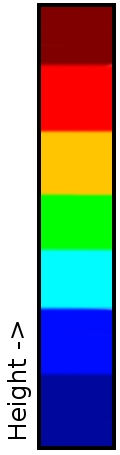
\includegraphics[scale=0.3]{images/HeightScale}}&&
			\subfloat[Increase and Decrease]{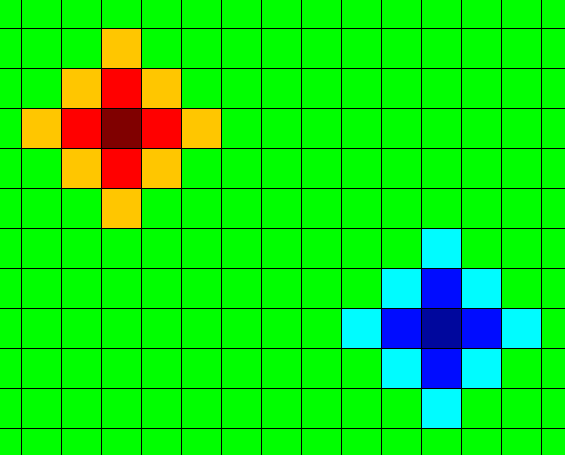
\includegraphics[scale=0.2]{images/Part1IncreaseAndDecreaseCharges}}&
			\subfloat[Decrease and Increase Combination]{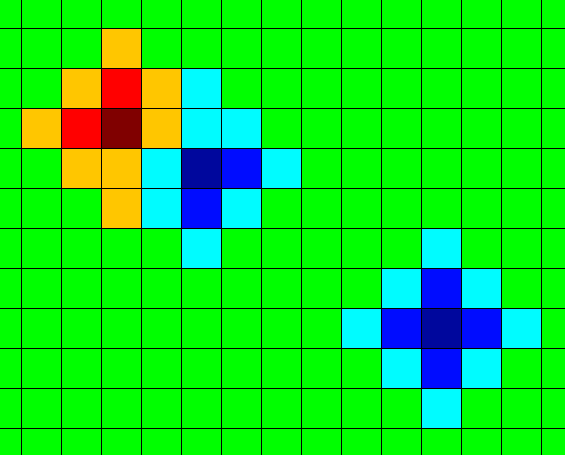
\includegraphics[scale=0.2]{images/Part2DecreaseCharge}}&
			\subfloat[Undo first Increase]{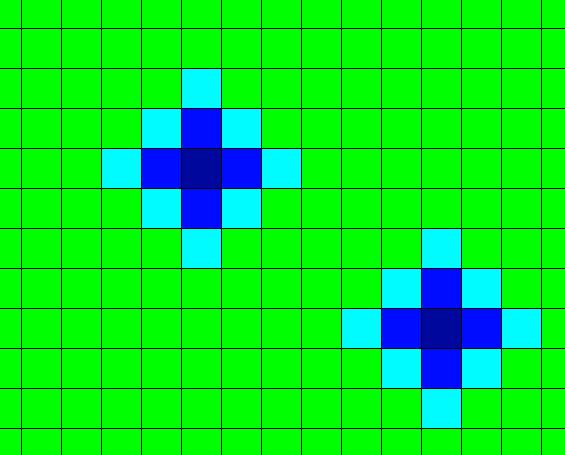
\includegraphics[scale=0.2]{images/Part3RemoveFirstCharge}}
	\end{tabular}
		\caption{Terrain Manipulation Example}
	\end{figure}
	
	\subsubsection{Action-Phase}
	Now we get to the practical part. After planning out the path by deforming the terrain the player now needs to move. Moving along hills makes us sliding and thus gaining or losing speed flexibly. The hill slopes influence our speed. We are equipped with a jetpack to alter our velocity for further increasing or decreasing our speed. The speed helps us getting further. If we are too slow we might lose. So raising the hills must be carefully considered in the first phase.
	There will be further obstacles like turrets that are distributed on the map. The player needs to avoid getting shot.
	\begin{figure}[ht]
		\centering
		\begin{tabular}{cccc}
			\subfloat[Start with no Speed]{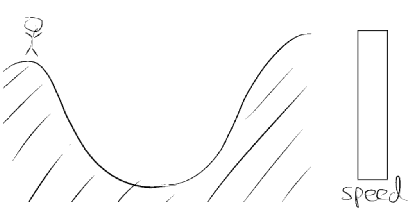
\includegraphics[scale=0.35]{images/StoryboardMovementPart1}}&
			\subfloat[Speed Increase due to Gravity]{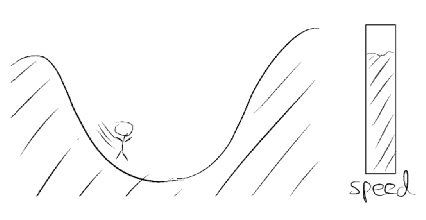
\includegraphics[scale=0.35]{images/StoryboardMovementPart2}}&
			\subfloat[Speed Decrease due to Gravity]{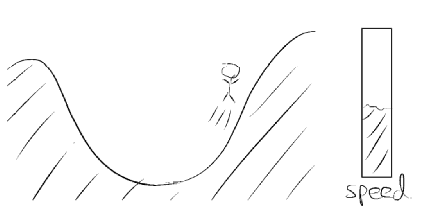
\includegraphics[scale=0.35]{images/StoryboardMovementPart3}}&
			\subfloat[No Speed after short Jetpack Boost]{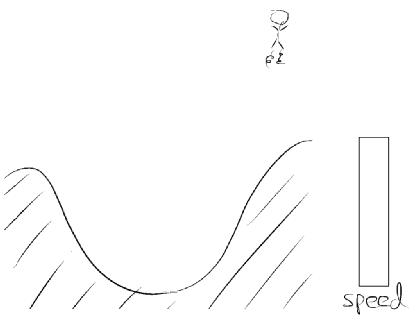
\includegraphics[scale=0.35]{images/StoryboardMovementPart4}}
		\end{tabular}
		\caption{Terrain Manipulation Example}
	\end{figure}
	
	\subsubsection{Terrain}
	From the development point of view the level designer not only creates terrains. The level designer must also define several certain areas that can be deformed by the player which will be discussed in the next section. The terrain looks different in each level. Sometimes we got a grassy landscape, or in other cases more rough plateaus. Some scenarios might be even windy and push the player softly around. At some points there will be water in the map as rivers, ponds or lakes. The fall damage is limited to the player's advantage at this point but on the other hand it slows the player down when he slides on it. If the player's speed is too low one might even dive. Grassy areas cause slight frictions so therefore decelerate the player a little bit. Ice causes no friction and rubble areas have very high friction.
	These areas are firstly flat or already hills or valleys according to the default terrain one gets. The player moves the mouse over the whole terrain in the first gaming phase. Deformable areas will be highlighted by blinking, coloring and or sound effects. Once the player picked an area and clicked on it this area raises up to a hill or lowers down to a valley. The longer one hold the mouse button the more the area gets deformed. And this procedure needs to be done until the player thinks he might be able to reach the goal in the second phase. So the whole process of finding or building the path is like solving a puzzle.
	What is being actually changed is the y-value of the terrain and the radius.
	It is possible to change the terrain several times until the player is ready to try it out. Areas that can not be manipulated will be identifiable as colored districts.
	Then in the next phase the player starts with a default speed value. When he slides along the hill the character we are playing accelerates due to physical laws. These accelerations raise the speed. The gained additional speed is crucial to getting further. Didn't the character gain enough speed the slope of the hill was not well considered first. The other case would be if the character is too fast after passing a hill.
	In the upcoming levels the player will be more and more restricted of deforming the terrain so reaching the goal will be more and more difficult.
	
	\subsubsection{Character}
	The player's character is a guy wearing a jetpack and riding on skis. The character's health will be displayed as a health bar. The health bar changes in several cases. It includes fall-damage that depends on relative vectors of slope normals and the velocity. Also when undergoing explosive damages or getting hit by turrets. There again different types of turrets causing other amounts of damage, like rocket-based, impulse-based and laser-based turrets. It's jetpack can be loaded by collecting fuel packs during the entire level so fuel bars will be also displayed.
	The movements of the character changes as the consistencies of different terrains influence the velocity of the character. More on that on the terrain section.
	According to how much the area the player is sliding on is curved, the player can also slide sideways. Either slightly, fully or also not at all.
	The player won't be able to shoot unless he finds gadgets that allow him to do so.
	The player has not infinite trials to deform the terrain. He has for example 5 charges and thus can make 5 changes on the terrain.
	Also the player can place helpers during the manipulation phase. These helper are mines, fuel tanks or other objects that could help him reach the goal.
	
	\subsubsection{Camera}
	There are two kinds of cameras: Planning Camera and Ingame Camera. The planning camera provides an overview so the player will be able to look down at the whole terrain from the top. Also the camera can be zoomed in and is rotateable so eventually one gets six degrees of freedom to move the camera around.
	The ingame camera can be switched between ego perspective and third person. It depends on the model quality and shall make the gameplay more comfortable for the player.
	
	\subsubsection{Obstacles}
	Depending on the terrain or the whole scenarios, obstacles could be turrets that try to shoot the character. There are different types of turrets causing other amounts of damage, like rocket-based, impulse-based and laser-based turrets. Or just borders or even gates that stay on the player's way. A further classification of obstacle types are natural background obstacles like wind. Windy areas might push the player softly around and of course influence his speed.
	
	\subsubsection{Gadgets}
	The borders from the obstacles-section can also be doors or gates. During the first phase the player should not only concentrate on the goal itself since the straight path to it might not be necessarily the correct one. Possible gadgets are keys that open gates. Further gadgets are grappling hooks to get to platforms that are not reachable otherwise. In the manipulation phase-section was mentioned that the player can place walls to run on. But to be able to do that one needs to collect special boots first which are positioned somewhere in the terrain. This again depends on the terrain consistency. Metallic grounds give metallic walls. In this case the player needs to collect magnetic boots. Each wall type provides running in each direction.
	
	\subsection{Technical Achievement}
	Our focus on technical achievement is the manipulation of the terrain or level in real time by the player to manipulate the speed he is gaining or losing constantly.
	To achieve that from the development point of view we get access to the heightmap and modify it. Then the terrain geometry and respective textures can be updated when the player changes the terrain. Changing is done easily as the ingame tool has very few parameters such as radius, amount and changing the +y-value of the terrain for raising and -y-value for lowering.
	As mentioned at the very beginning of the game description-section modifiable or restricted areas of terrain are highlighted. For example a sound effect starts, the area is colored when hovering the mouse over it or the area blinks.
	
	\newpage
	\subsection{Big Idea Bullseye}
	\begin{figure}[ht]
		\centering
		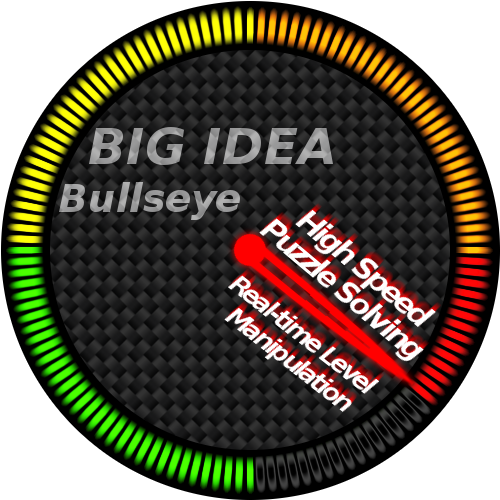
\includegraphics[scale=0.7]{images/bigIdeaBullseye}
		\caption{Big Idea Bullseye Image}
		\label{bigIdeaBullseye}
	\end{figure}
	
	\subsection{Tasks}
	
	\subsubsection{Development Schedule}
	The exploded development schedule for the project can be seen in Figure \ref{developmentSchedule} or in the attached image.
		\begin{figure}[H]
			\centering
			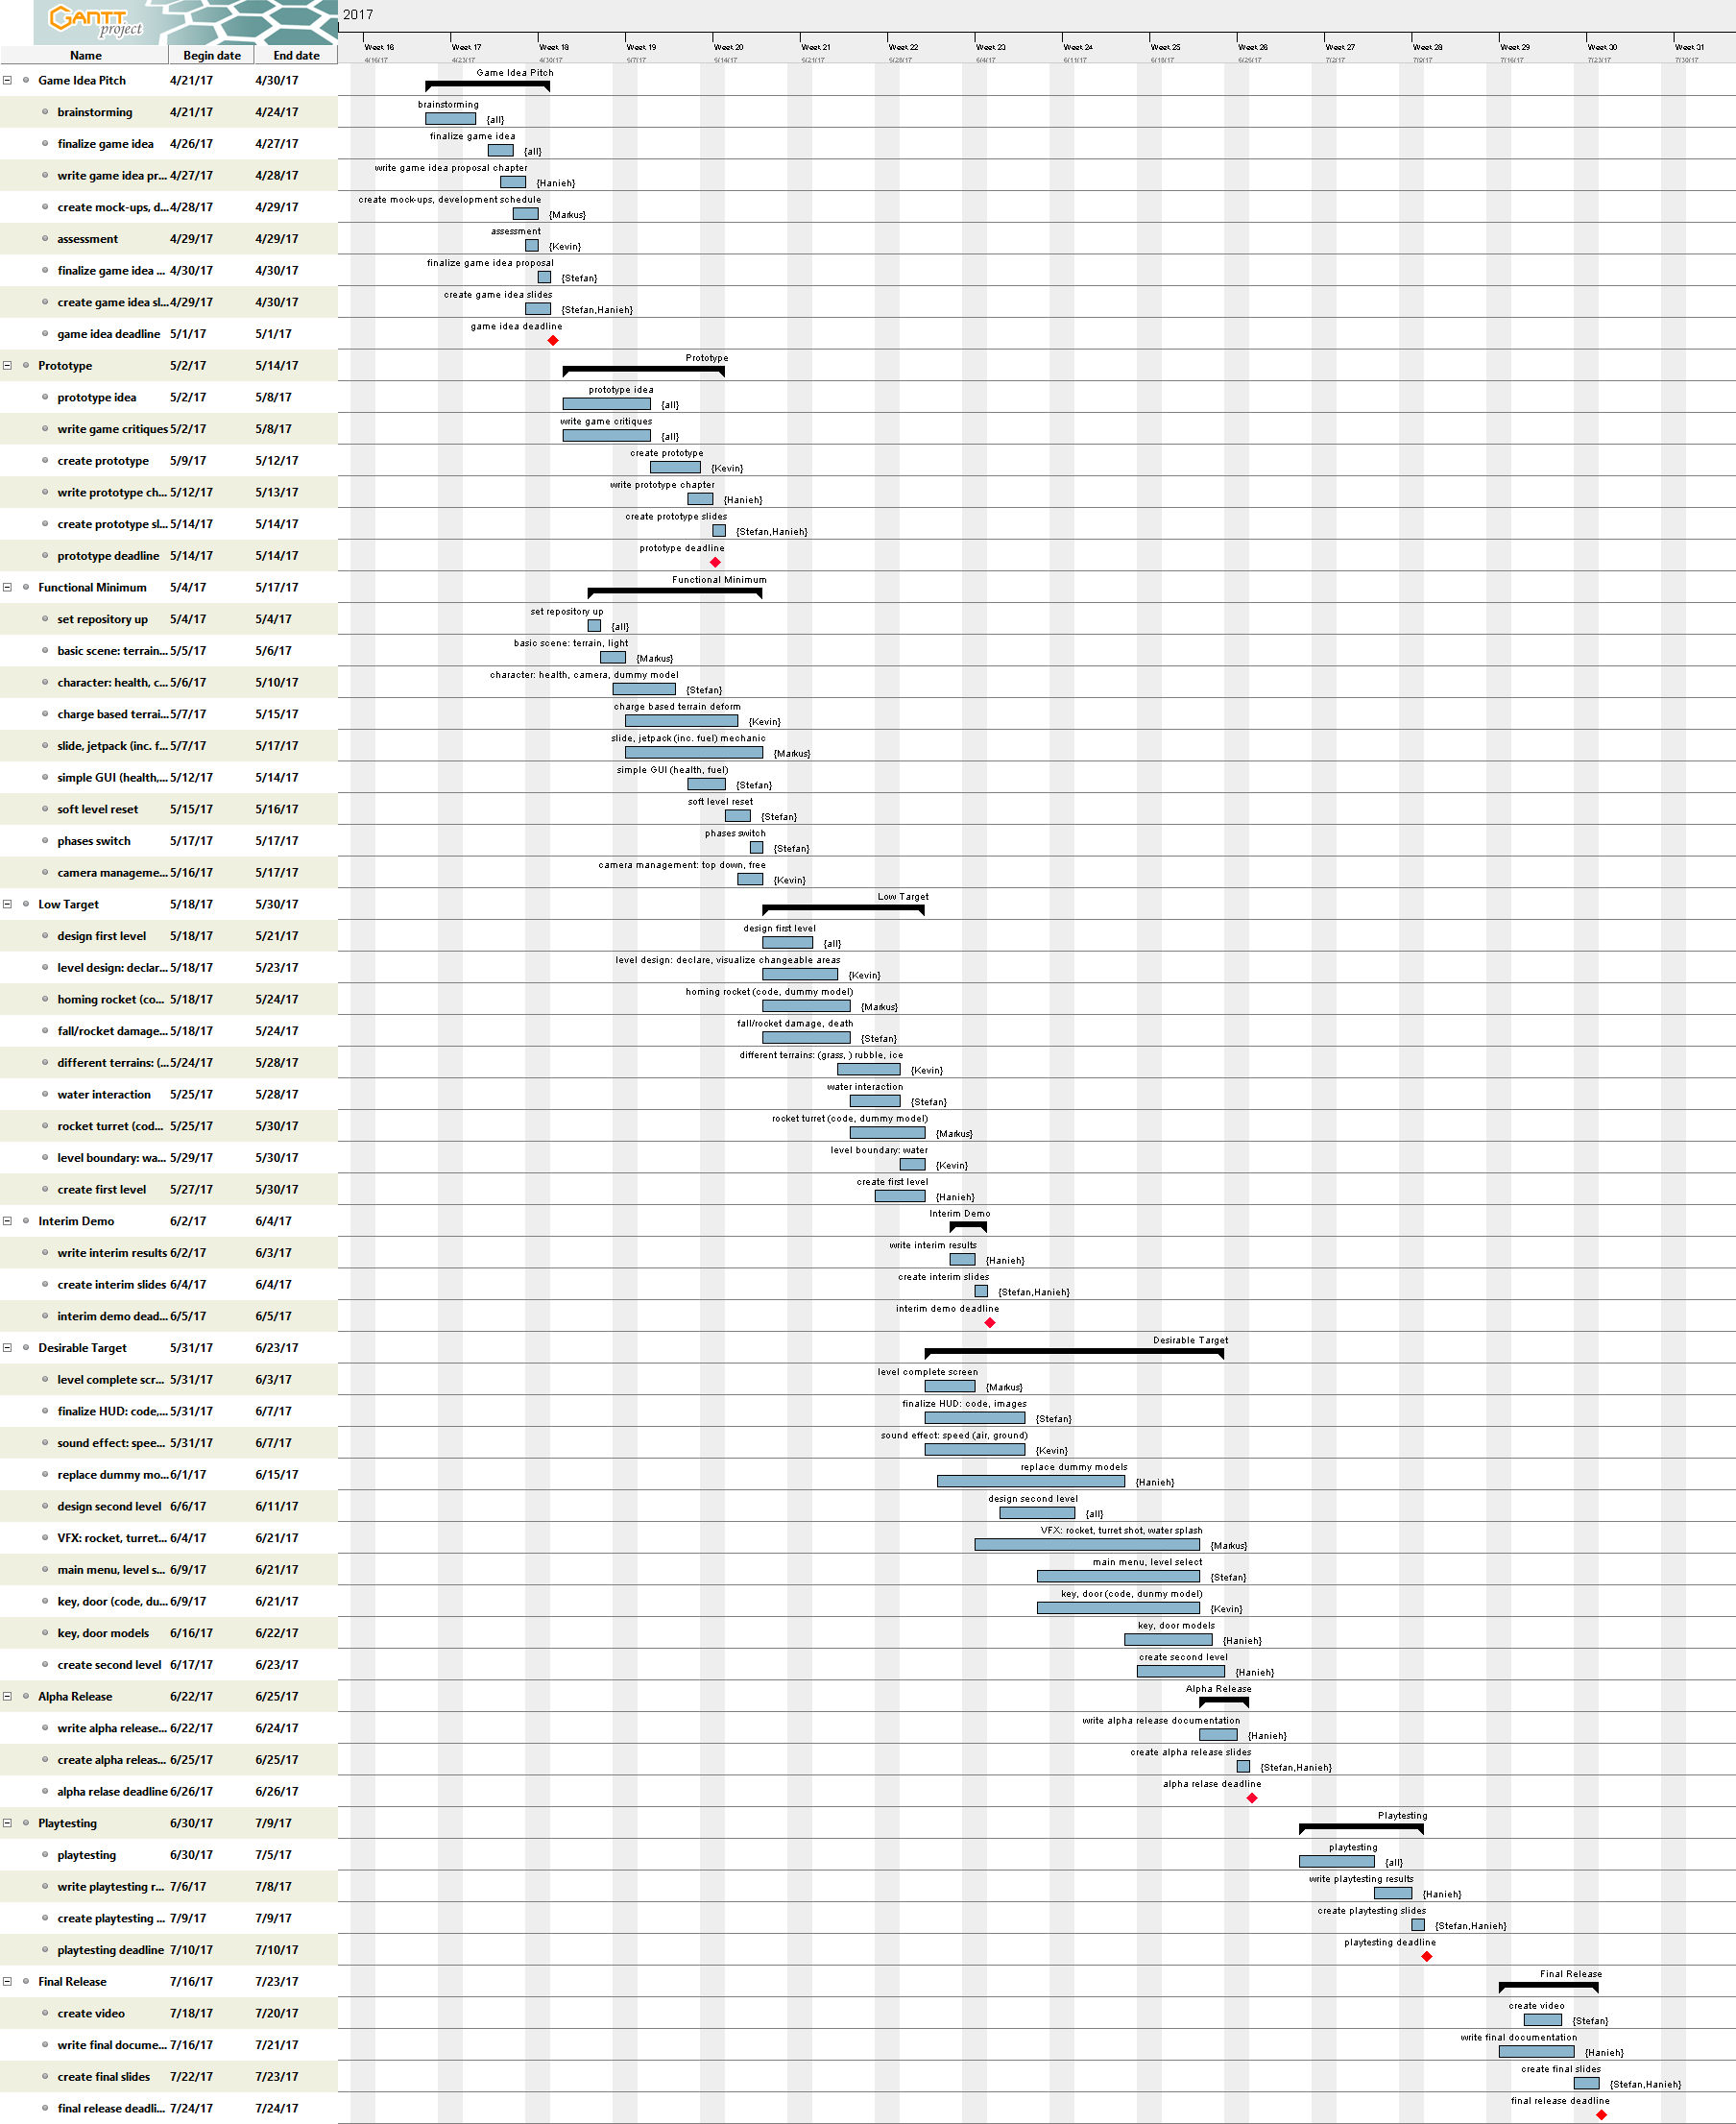
\includegraphics[height=\textheight]{images/GamesLab2017SS}
			\caption{Development Schedule}
			\label{developmentSchedule}
		\end{figure}
		
	\subsubsection{High Target}
	\begin{itemize}
		\setlength\itemsep{0.1pt}
		\item sound effects: rocket, death, goal, taking damage, sliding
		\item time based obstacles
		\item different turrets: impulse, plasma
		\item grappling hook, flying objects
		\item more levels
	\end{itemize}
	
	\subsubsection{Extras}
	\begin{itemize}
		\setlength\itemsep{0.1pt}
		\item background music
		\item level designer for player
		\item target shooting
		\item manipulation of terrain during action phase (slowmotion)
		\item other gadgets
	\end{itemize}
	
	\subsection{Assessment}
	The game is a strategic puzzle game with action elements. The main strength will be the interaction between the manipulation and the action phase. In the manipulation phase you can change the height of several areas of the map in a way that benefits you in the second phase. In the action phase you can slide along hills and use different gadgets to get to your destination and solve the puzzle. The big challenge will be to manipulate the map in a way where you can slide with the right amount of speed to get to your destination.
	This kind of game will most likely appeal to a puzzle games liking or strategic thinking audience. But casual players could also be interested in such a game because of the fast paced action phase.
	An important part will be to make interesting puzzles which will be challenging to solve. So that the player has to think about which terrains to manipulate and how. But also be very careful at which point in time he/she uses the available gadgets.
	
	\newpage
	\newpage
	\section{Game Prototype}
	\subsection{Introduction}
	Our idea is to create a game where the player needs to deform a terrain in order to gain speed due to physical laws. The game consists of two phases: The manipulation and the action phase.
	In the first phase, the manipulation phase, the player has to deform the terrain to his advantage. He can create hills or place gadgets like fuel tanks. When he raises the terrain at a certain point he gets hills. And the hills again provides certain slopes which are important for the next phase. 
	In the action phase the player has to slide along the hills that he has created in the previous phase. The slopes of the hills have an important influence on the speed and cause a momentum that the player needs to reach the goal. If the speed is not high enough a helpful gadget like fuel tanks can help the player to compensate deviations or losses.
	So during manipulation phase the players needs to consider his steps very well and think strategically. And during the action phase his movements are based on physical laws so he needs to slide and move correctly along.
	
	\subsection{Game Rules}
	During the manipulation phase the player can not deform the terrain as much as he wants. He gets a certain amount of charges. E.g. five charges mean, that the player has five possibilities to deform the terrain. 
	Besides the charges he has also a certain amount of fuel tanks that he is allowed to use. For example two fuel tanks simply mean that he can place two fuel tanks all over the terrain except for the restricted areas. Using a fuel tank meant to be able to move about 5 cm in each direction.
	Turning this idea into a prototype we decided to make a sandbox. We crafted a box made out of wood and filled it with sand.
	\begin{figure}[H]
		\centering
		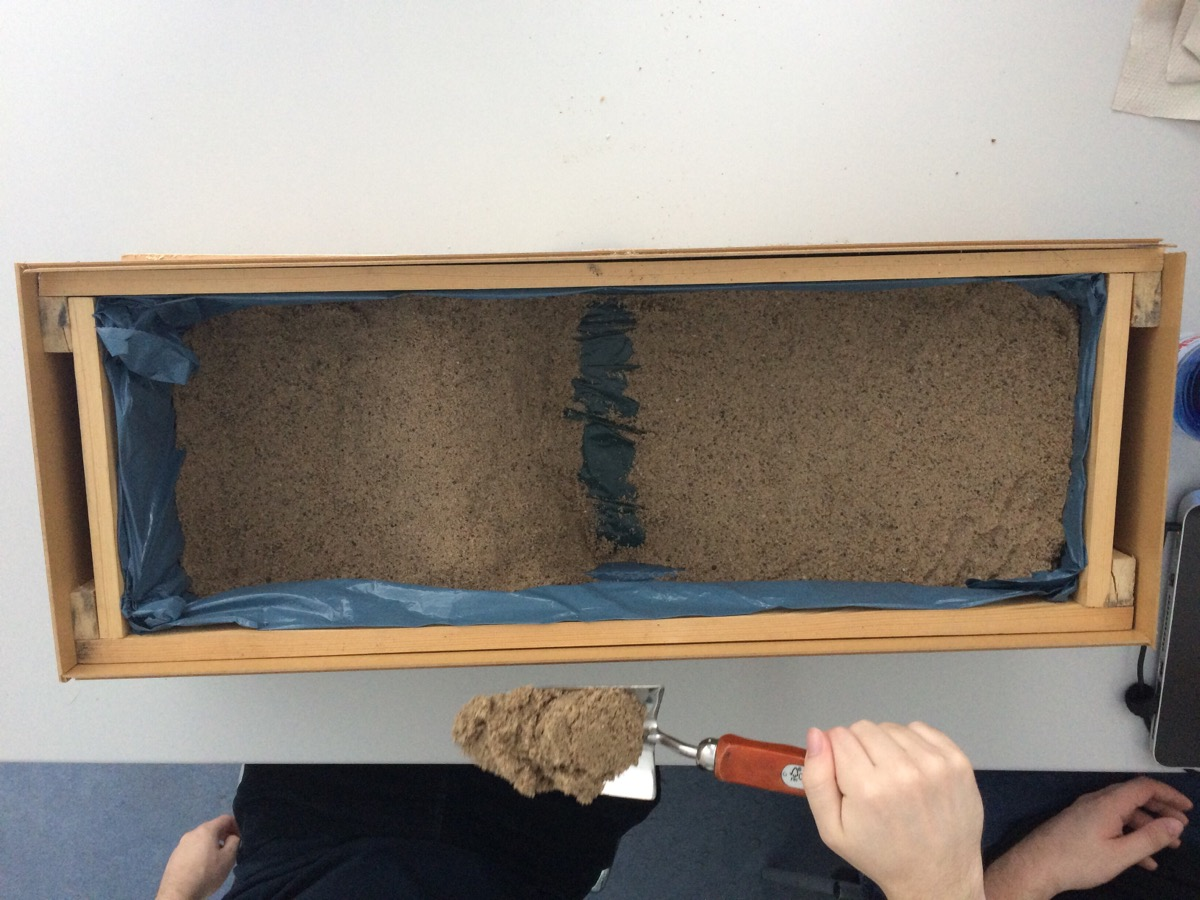
\includegraphics[scale=.2]{images/prototype/prototypeOverview}
		\caption{Prototype Overview}
		\label{prototypeOverview}
	\end{figure}
	During the manipulation phase we shaped the sand and made some hills. For fuel tanks we just cut some papers.
	\begin{figure}[H]
		\centering
		\begin{tabular}{cc}
			\subfloat[Example Hill]{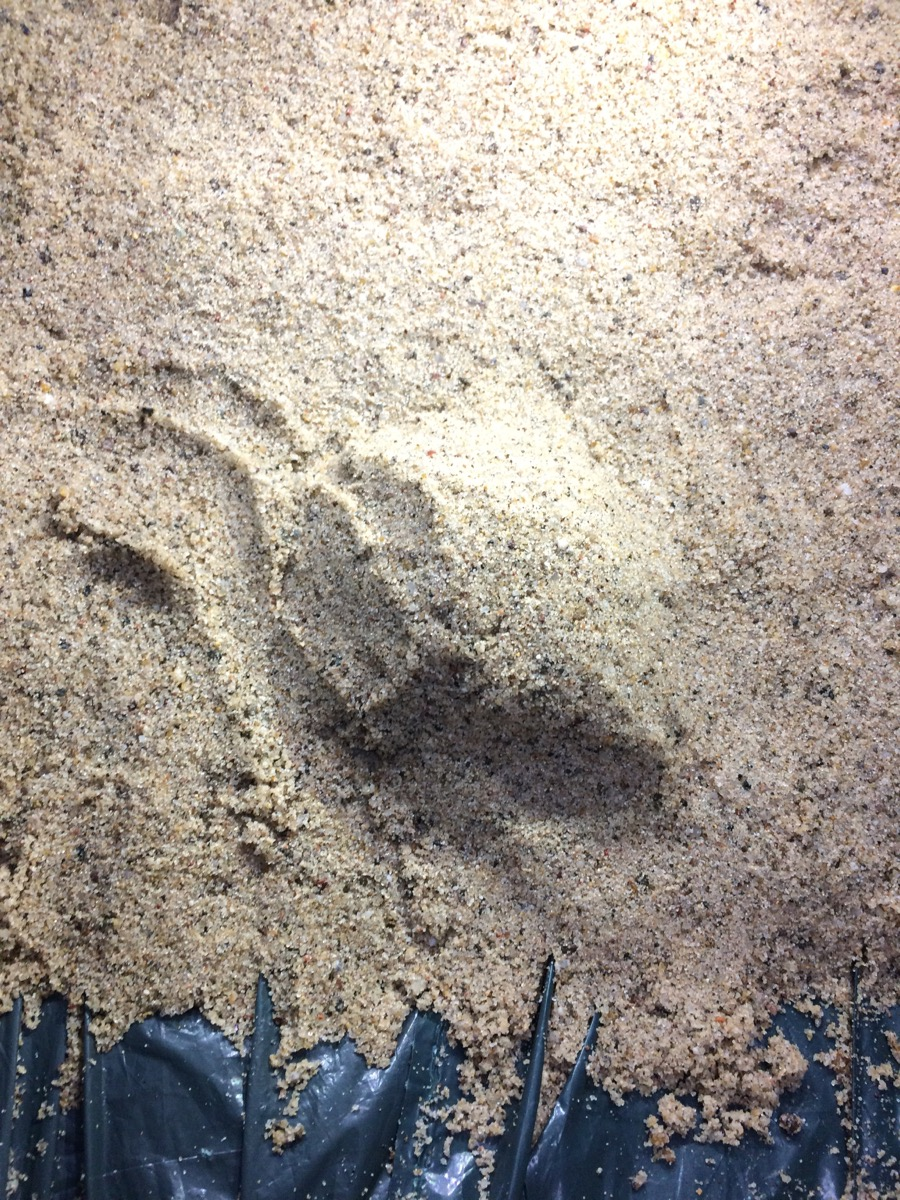
\includegraphics[scale=0.2]{images/prototype/prototypeHill}}&
			\subfloat[Fuel Tanks]{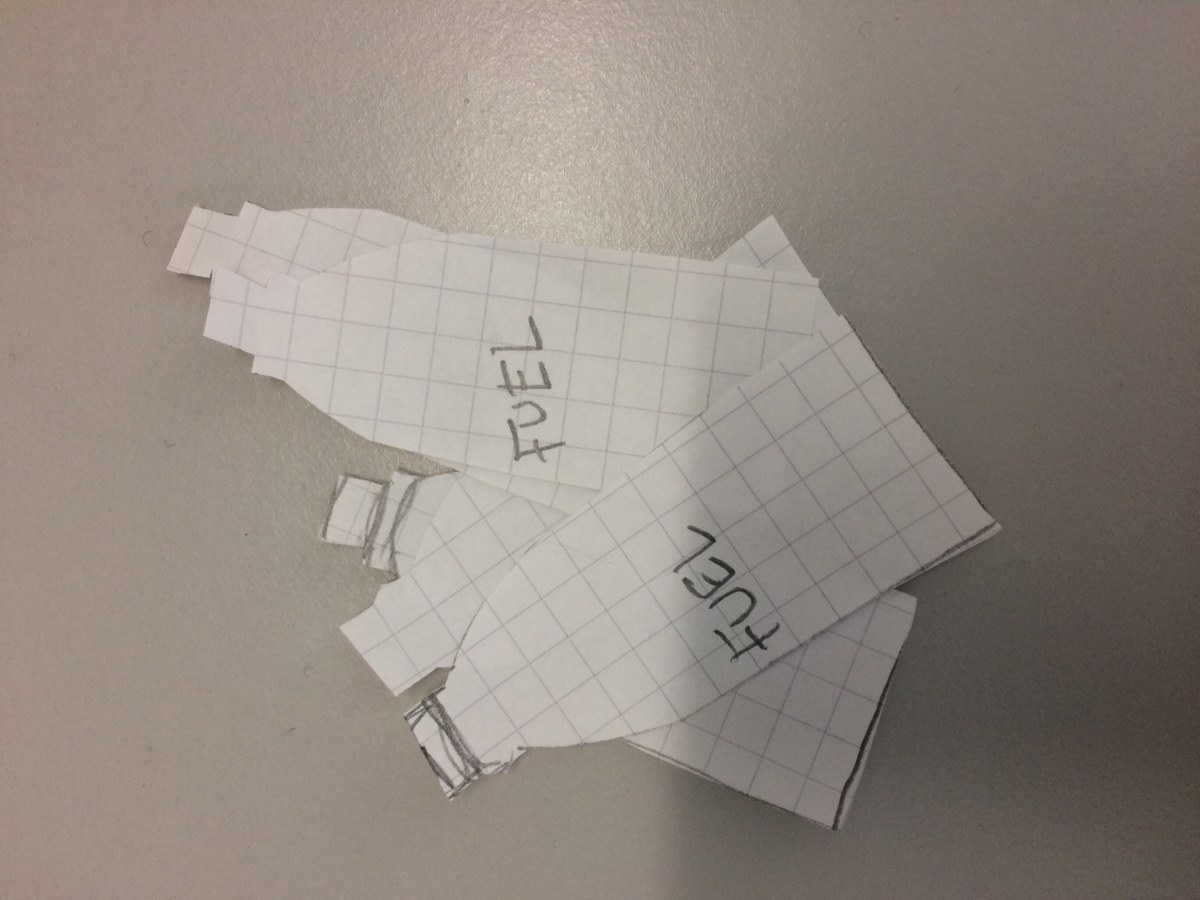
\includegraphics[scale=0.2]{images//prototype/prototypeFuelTanks}}
		\end{tabular}
		\caption{Prototype Explanation}
	\end{figure}
	The character is represented by a marble. In the first step we start at an arbitrary point and then roll down towards the first point that we decided to deform. Sliding along the hill gives us speed to overcome the deadly valley.
	\begin{figure}[H]
		\centering
		\begin{tabular}{ccc}
			\subfloat[Timestep 1]{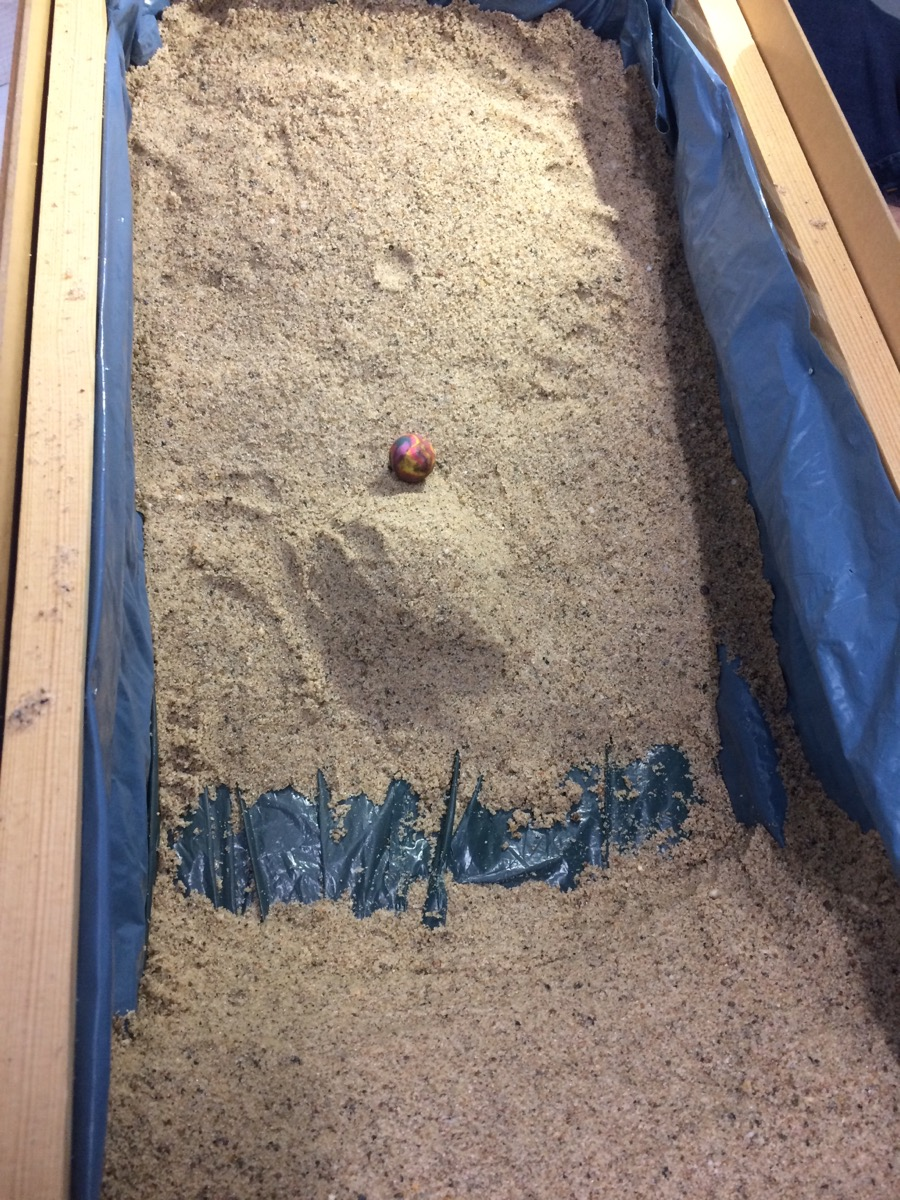
\includegraphics[scale=0.13]{images/prototype/prototypePlaythrough_1_1}}&
			\subfloat[Timestep 2]{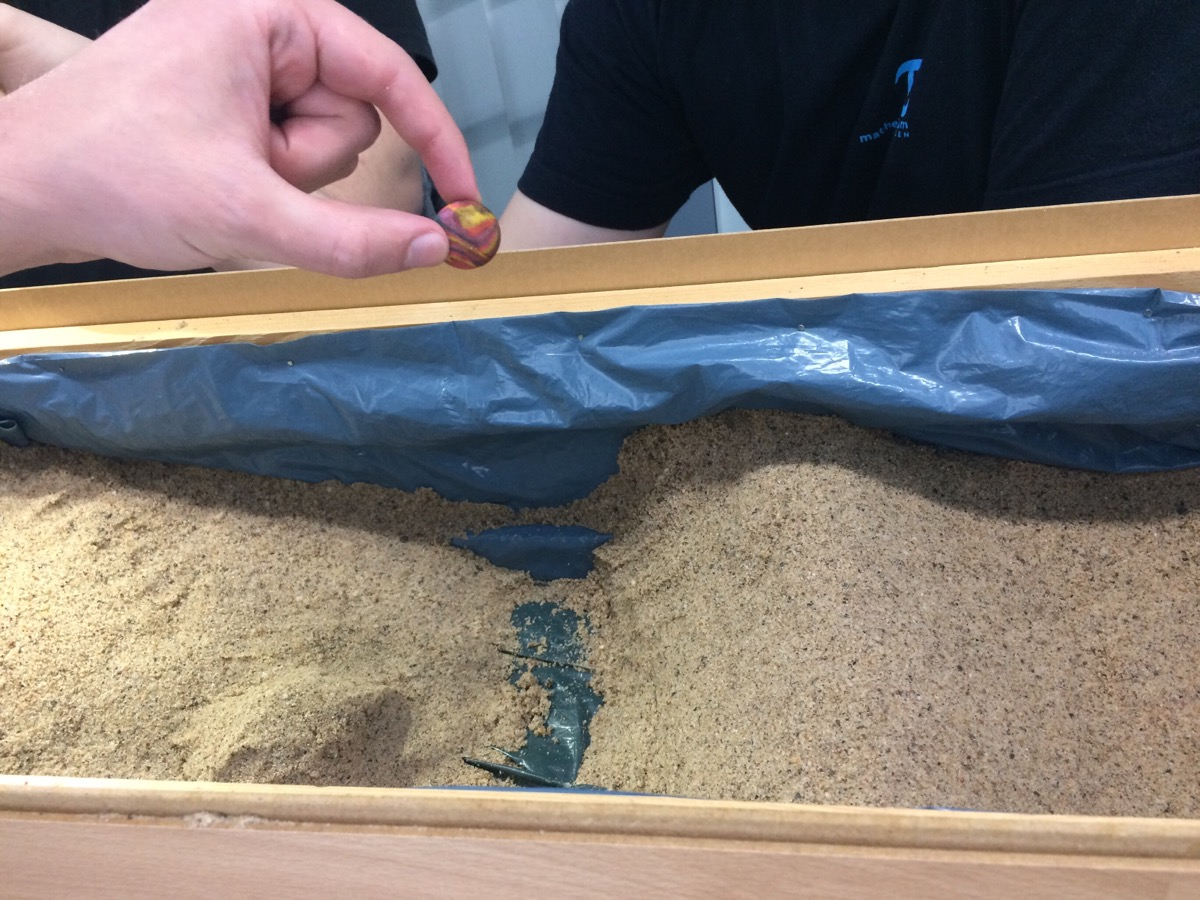
\includegraphics[scale=0.13]{images/prototype/prototypePlaythrough_1_2}}&
			\subfloat[Timestep 3]{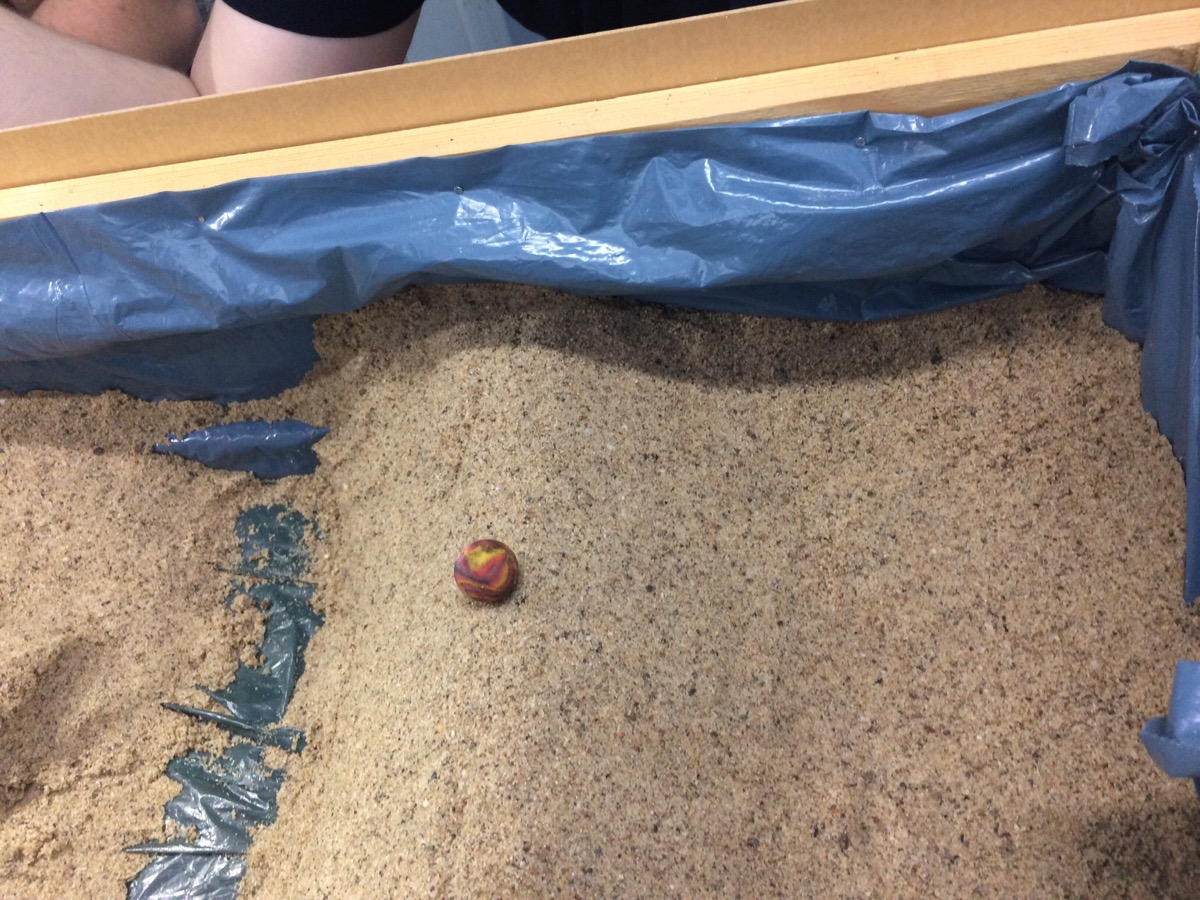
\includegraphics[scale=0.13]{images//prototype/prototypePlaythrough_1_3}}
		\end{tabular}
		\caption{First Level}
	\end{figure}
	It was hard to simulate the acceleration since sand was not an optimal ground due to high friction. But still sand was a good decision when one wanted to deform the terrain.
	
	\subsection{Experience}
	Level design won't be easy since we will need quite a lot time to invent some good levels. It was a challenge to create a puzzle that was fair balanced between easy and hard. One of the remarkable experiences was the fact that the player needed a lot more time to solve the puzzle than we needed to create it. For comparison we needed about five to at most ten minutes to create a simple puzzle. But the player needed about twenty minutes to find a way to reach the goal. This tells us how different the chains of thought between the level designer and the player can be. 
	
	Three of us designed the level while the other person left for a while. One side of the terrain was lower than the other side. Unfortunately this is not identifiable on the pictures. On the higher area we put a wall. Almost one half of the wall soared above the lower area. At this point the player wouldn't be able to jump. The pencil marks the start point and the ball pen marks the goal. 
	\begin{figure}[H]
		\centering
		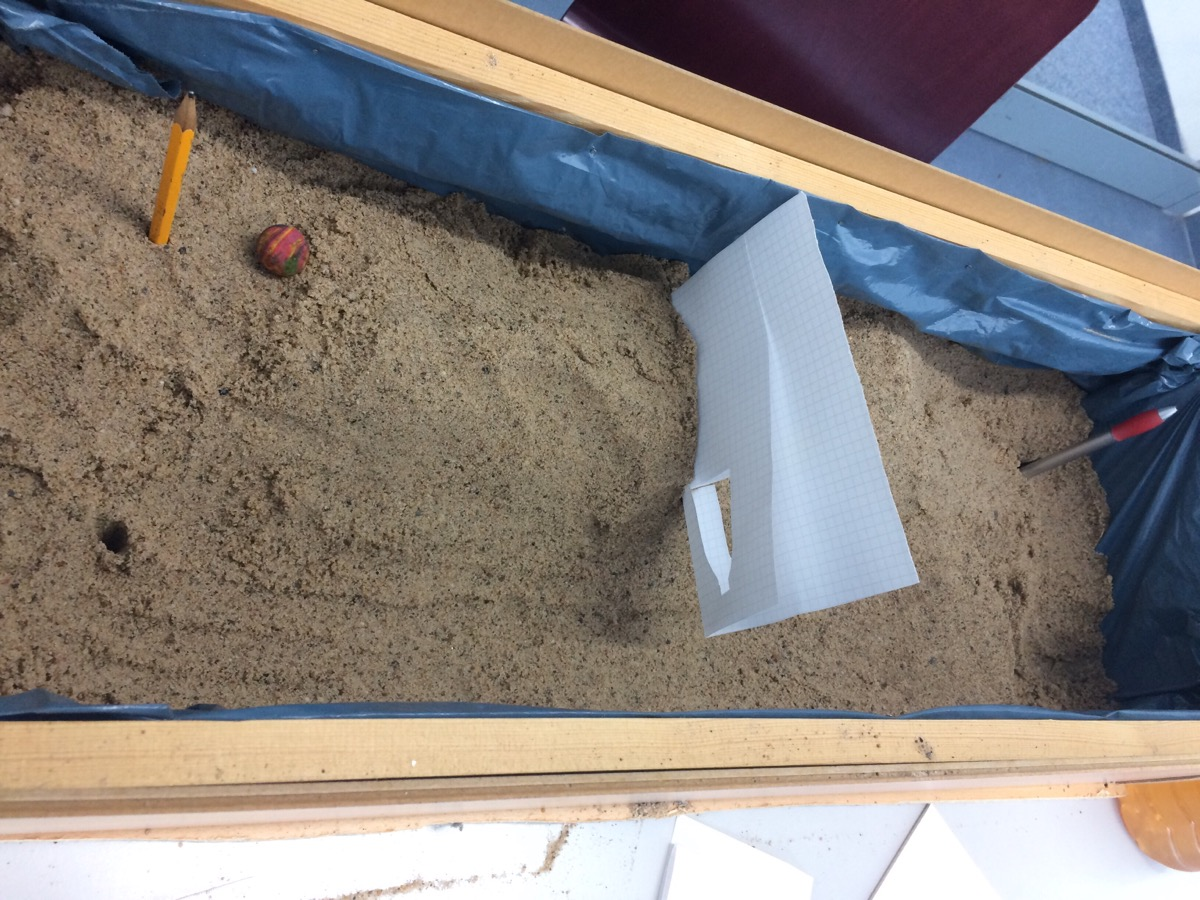
\includegraphics[scale=.2]{images/prototype/prototypeTerrain2}
		\caption{Second Terrain}
	\end{figure}
	Then the player came and started to play. We allowed him to have two charges and one fuel tank. 
	Entering the manipulation phase he firstly placed the fuel tank.
	\begin{figure}[H]
		\centering
		\begin{tabular}{cc}
			\subfloat[Experimenting]{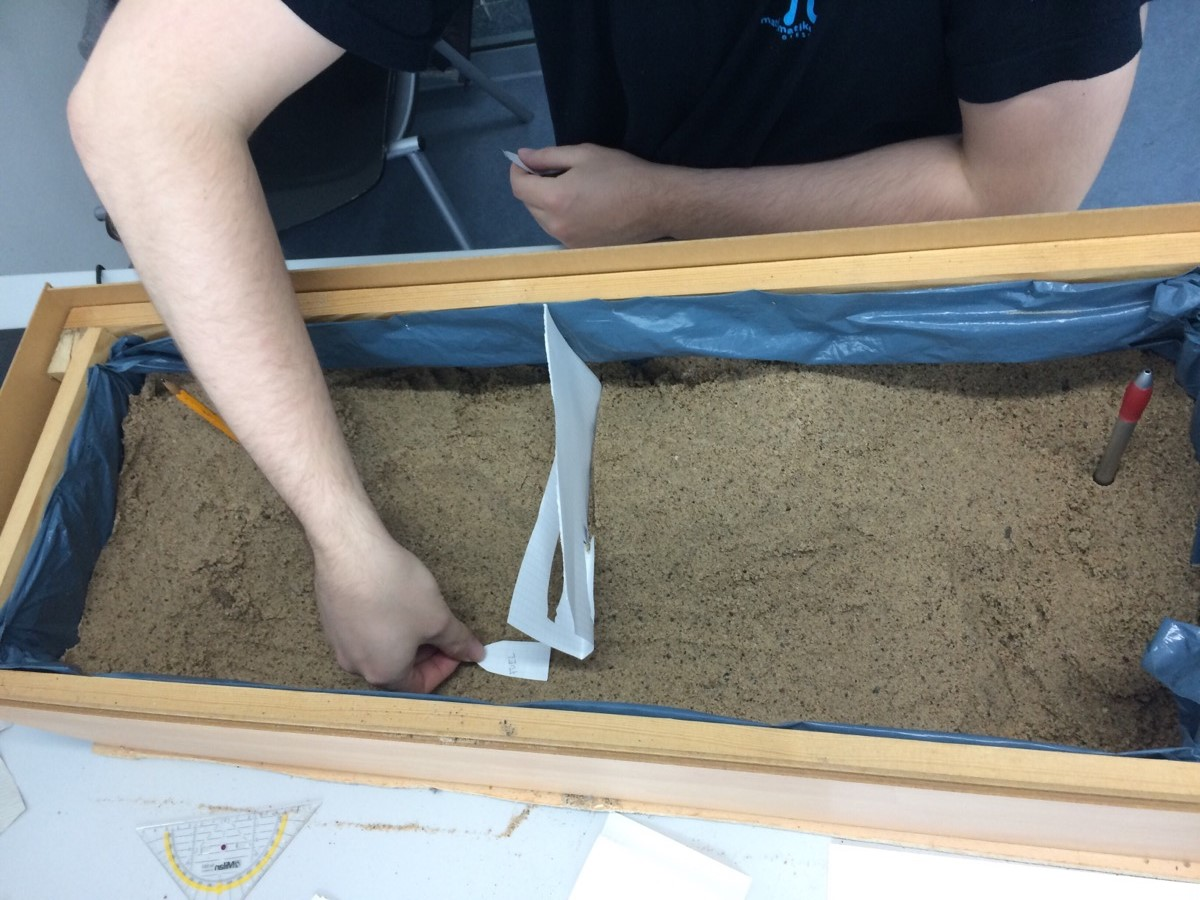
\includegraphics[scale=0.25]{images/prototype/prototypeFuelPlacements1}}&
			\subfloat[Final Location]{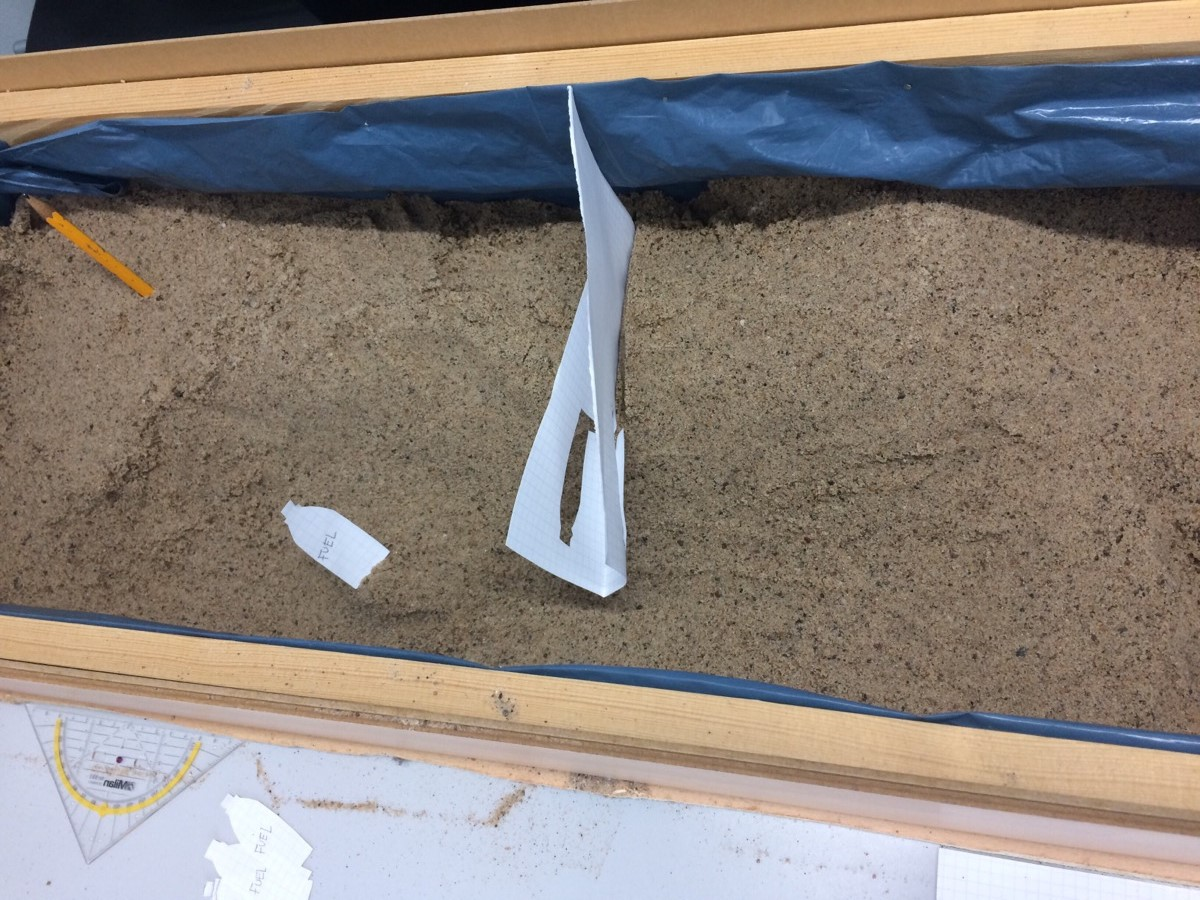
\includegraphics[scale=0.25]{images//prototype/prototypeFuelPlacements2}}
		\end{tabular}
		\caption{Fuel Tank Placement}
	\end{figure}
	Then after some deliberations he picked a spot for the hill. One of us, representing the CPU, built the hill for him.
	\begin{figure}[H]
		\centering
		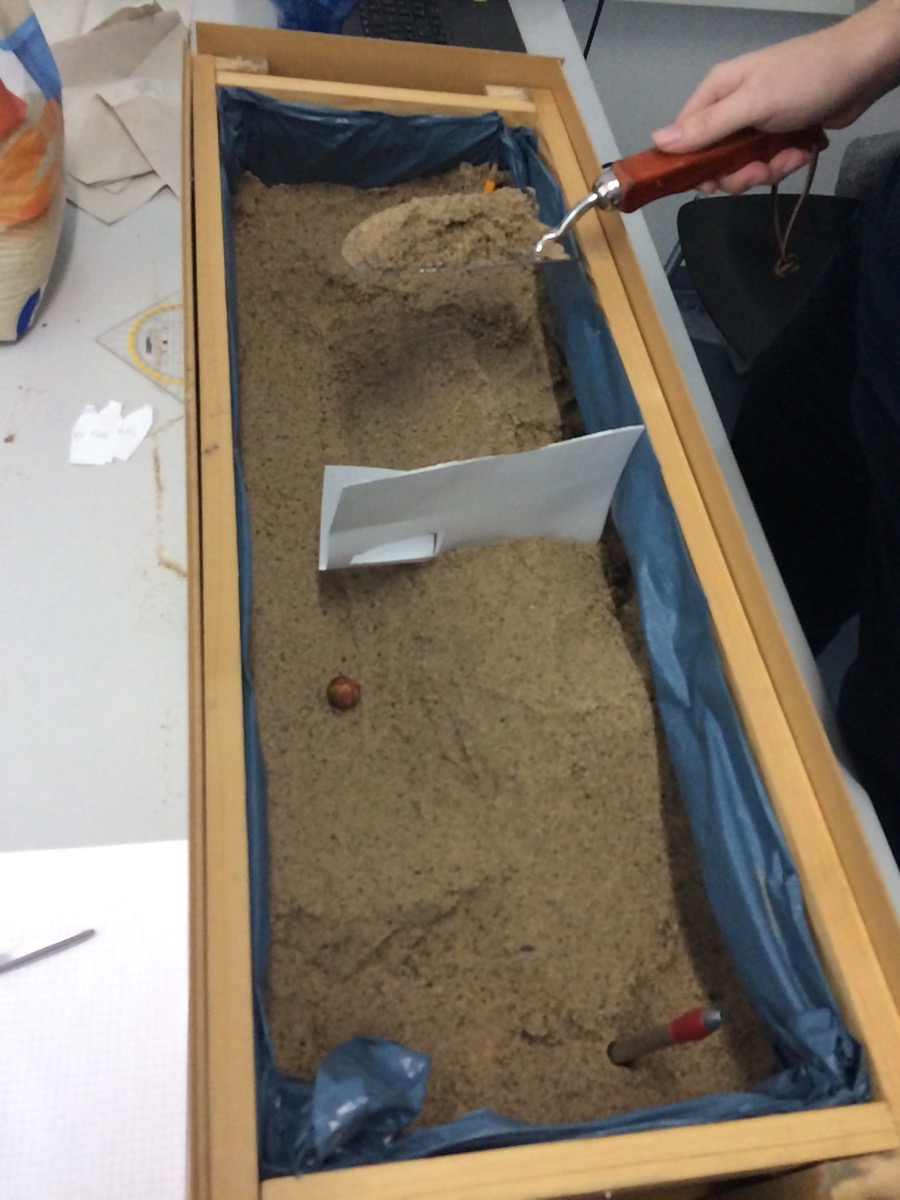
\includegraphics[scale=.2]{images/prototype/prototypeHill1}
		\caption{First Hill}
	\end{figure}
	But the player also decided to raise the same hill once gain because of the idea to gain more speed at the end by sliding along a higher hill.
	\begin{figure}[H]
		\centering
		\begin{tabular}{ccc}
			\subfloat[Step 1]{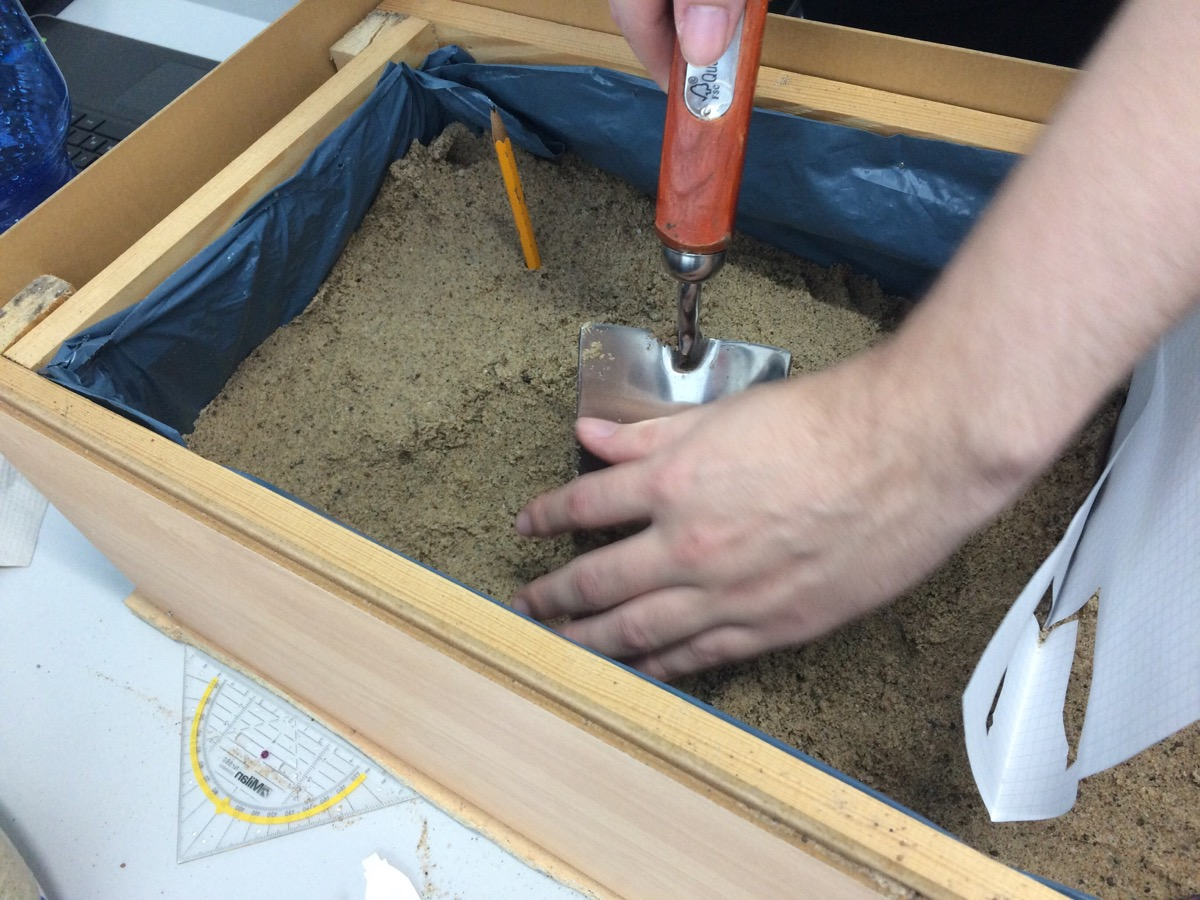
\includegraphics[scale=0.13]{images/prototype/prototypeHill2}}&
			\subfloat[Step 2]{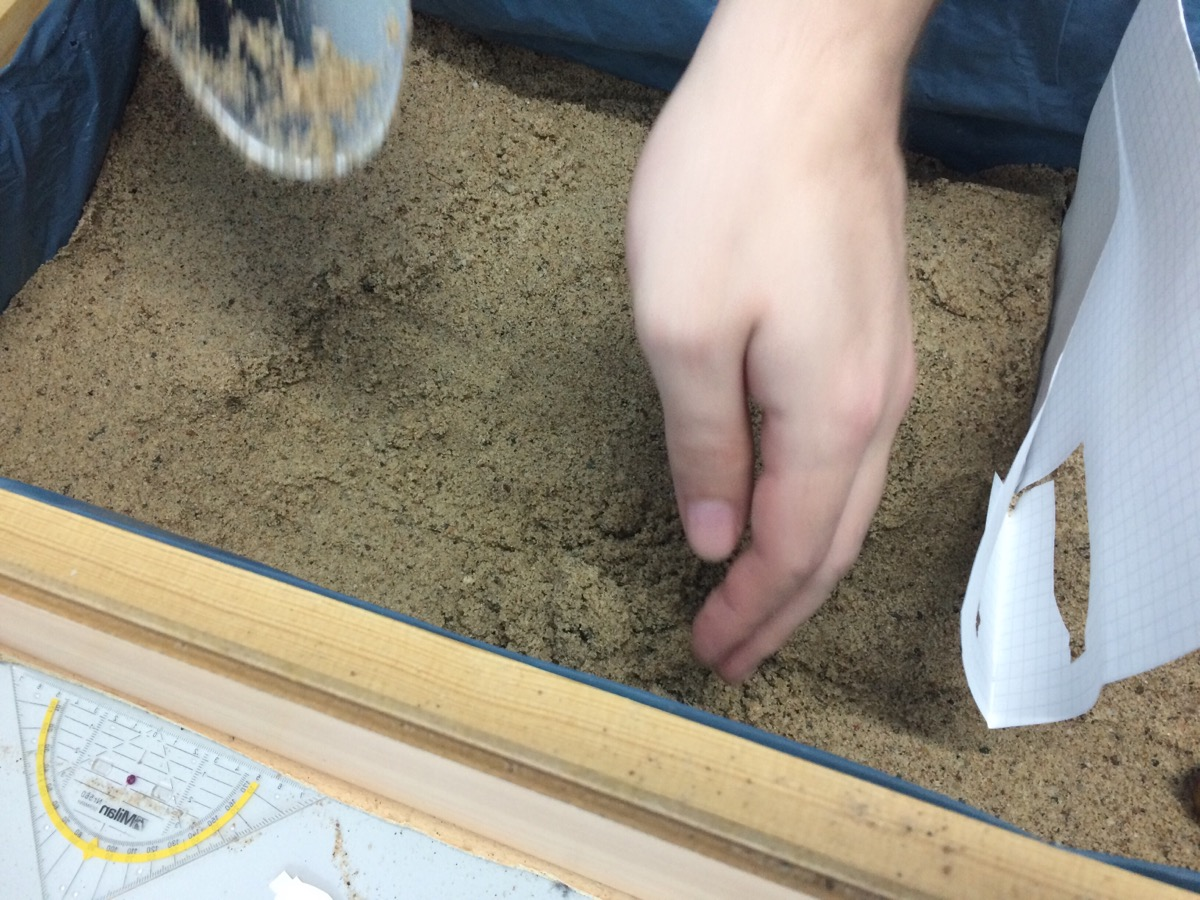
\includegraphics[scale=0.13]{images/prototype/prototypeHill3}}&
			\subfloat[Step 3]{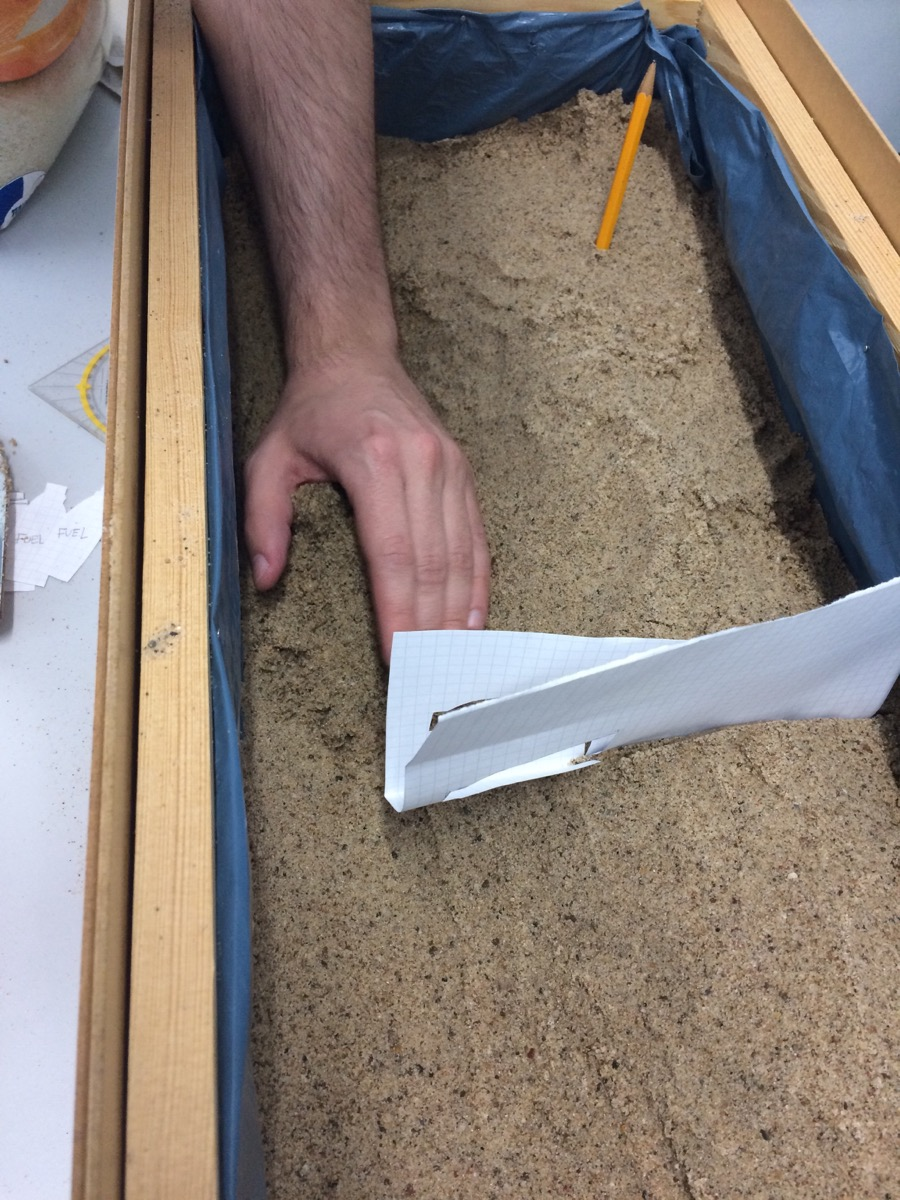
\includegraphics[scale=0.13]{images//prototype/prototypeHill4}}
		\end{tabular}
		\caption{Second Hill}
	\end{figure}
	When he was finished he initialized the action phase. He moved the marble to the fuel tank right onto the double hill. That made him get a high position from where he used the fuel tank. That made him fast enough to slide along the hill where the goal was set.
	\begin{figure}[H]
		\centering
		\begin{tabular}{cccc}
			\subfloat[Timestep 1]{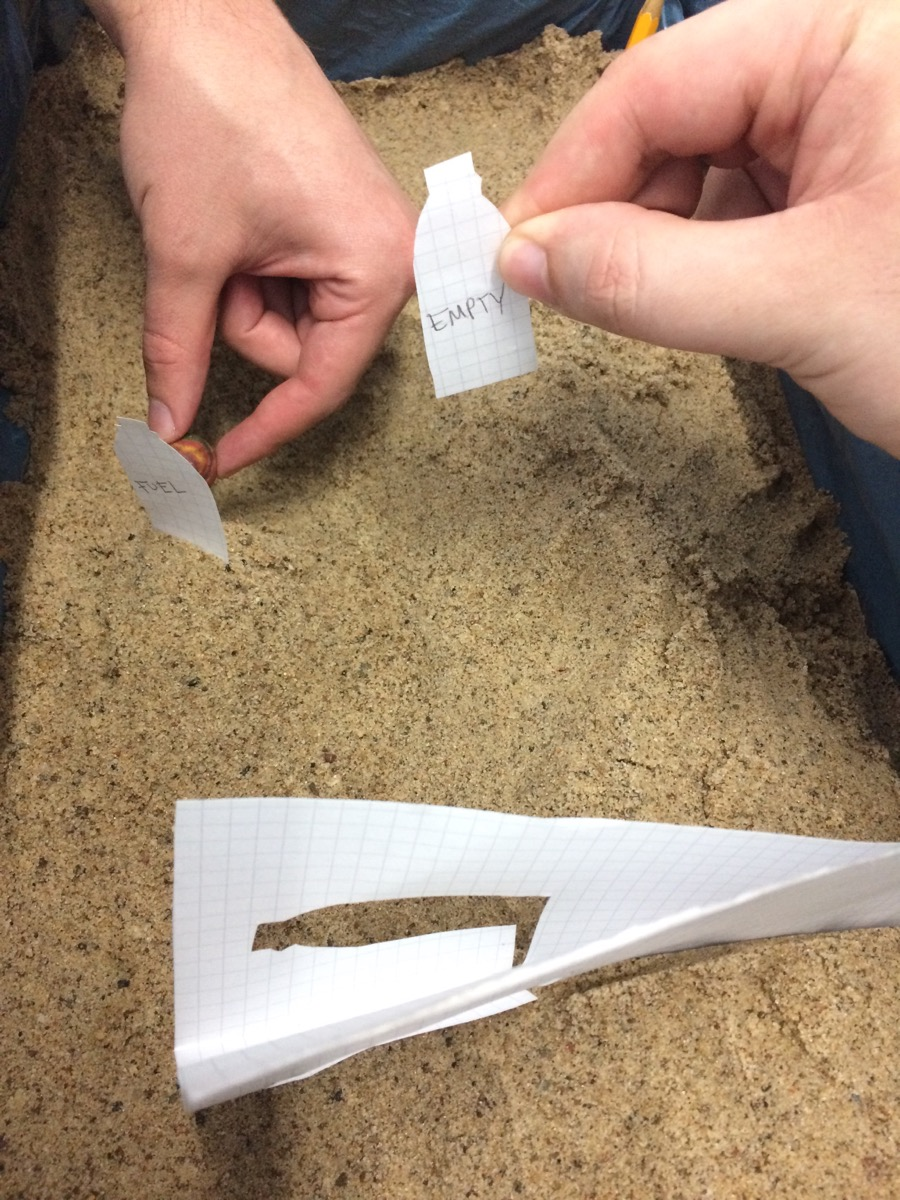
\includegraphics[scale=0.11]{images/prototype/prototypePlaythrough_2_1}}&
			\subfloat[Timestep 2]{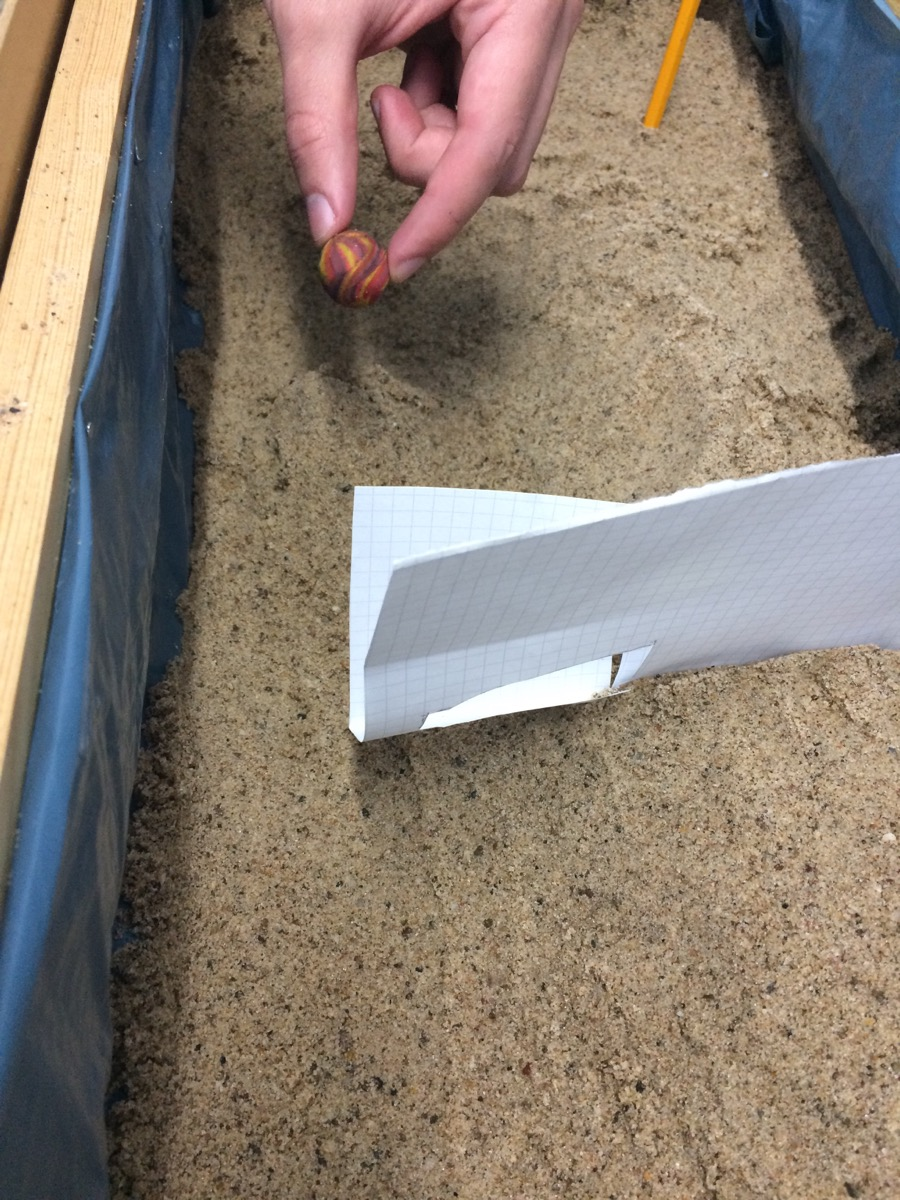
\includegraphics[scale=0.11]{images/prototype/prototypePlaythrough_2_2}}&
			\subfloat[Timestep 3]{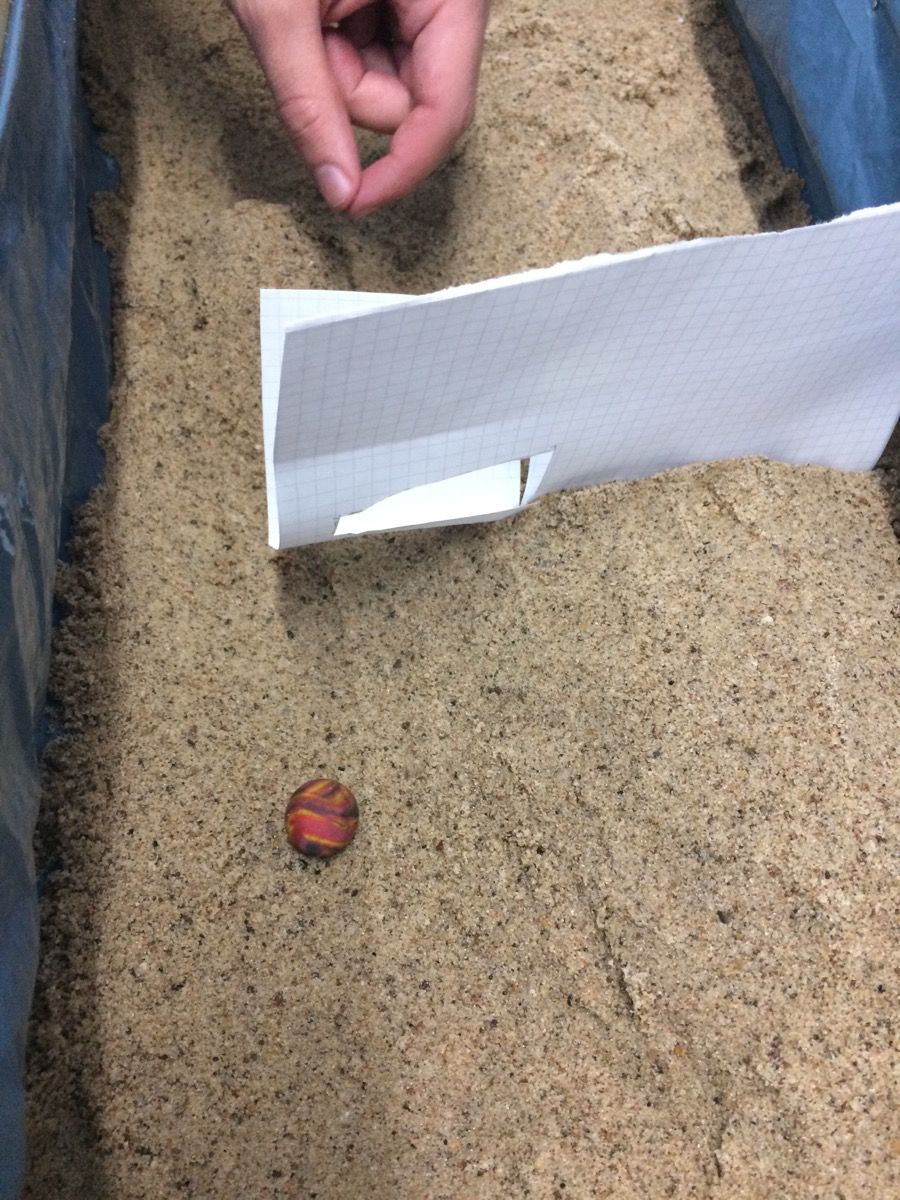
\includegraphics[scale=0.11]{images/prototype/prototypePlaythrough_2_3}}&
			\subfloat[Timestep 4]{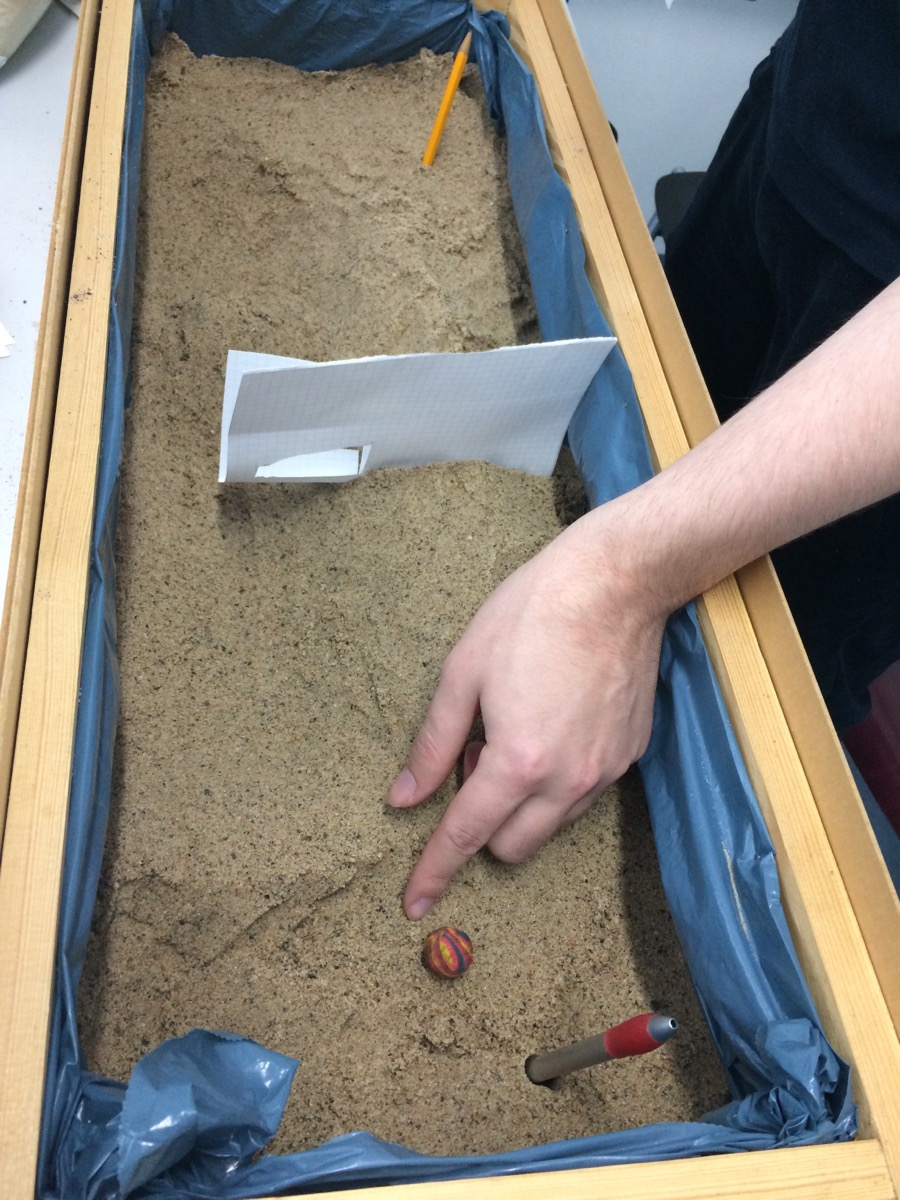
\includegraphics[scale=0.11]{images//prototype/prototypePlaythrough_2_4}}
		\end{tabular}
		\caption{Second Level}
	\end{figure}
	The player needed a few times to solve this problem. We will give the player infinite trials in the future as well.
	
	\subsection{What We Learned}
	Making a prototype means to make the game idea real and touchable. This helps us to get a better imagination and overview of what is in our mind. Deforming the hills with our hand made us better aware of good level designing. By actually touching the world we get a better idea of what could possibly be not logical or what could work. This also has the effect that we can share our imaginations better with other group members since everyone can see what is in our mind. This works better than just talking to the others. And during the discussion everyone can interact with one's imagination by touching our thoughts.
	
	And as already mentioned in the experience-section a further fact that we have learned is that the player needed a lot more time to solve the puzzle than we needed to create it. Having realized this time difference will help us to prevent avoidable mistakes.
	
	\subsection{Critiques}
	The manipulation of the terrain and also the level design will be our main focus of the game, because of the experiences we gathered from the prototype phase and also because it was very well received in the critiques.
	
	Many asked to merge the terrain manipulation into the action phase, but we will still keep it separated. Because it doesn't serve well to the whole puzzle idea and it would be more of an action game. Also it would make the terrain manipulation and the level design much more complicated.
	
	The idea of dynamic terrain is already in the making in the form of dynamic rivers/lakes. But it, along with turret destruction, will be a high target goal.
	
	A sandbox mode was asked, and we will make it in the form of a level editor, but it is set as an extra target.
	
	We will still keep a health bar, because that way we can make more turrets, also the player is able to make some mistakes without dying straight away.
	
	\newpage
	\section{Interims Report}
	\subsection{Functional Minimum}
	\label{sec:functionalMinimum}
	The focus of our functional minimum milestone was mainly on the most basic gameplay mechanics of our game and essential features that are need for it to be called a game. This meant both phases needed to be implemented, the Manipulation- as well as the Action-Phase. The Manipulation-Phase consisted of a controllable, floating top-down camera and the actual manipulation of our terrain. The Action-Phase contained the sliding movement and jetpack mechanic. Another very basic feature was some kind of user interface, which was realized by some text with numbers.
	
	\subsubsection{Basic Character Implementation}
	For both the functional minimum, as well as the low target, the character was represented by a capsule model which was provided by Unity itself. This enabled collision detection and shadow casting and will be easily replaceable with a real and animated model in the desired target. Also part of the basic character was a first person camera, which was a breeze to implement. Another essential aspect of the character script was handling keyboard and mouse input from the player. The basic control scheme is using the mouse to look around in first- and third person view, pressing “WASD” for slightly moving on the ground and in the air, holding down the spacebar to activate the jetpack and pressing enter to switch between both phases.
	
	\subsubsection{User Interface}
	As mentioned in Section \ref{sec:functionalMinimum} the user interface only consists of text with numbers for now (see figure \ref{fig:screenshot}). The displayed information changes depending on the current phase the player is in. In the Manipulation-Phase he can see the amount of charges he has left and in the Action-Phase he can see his current health and remaining fuel.
	\begin{figure}
		%\centering
		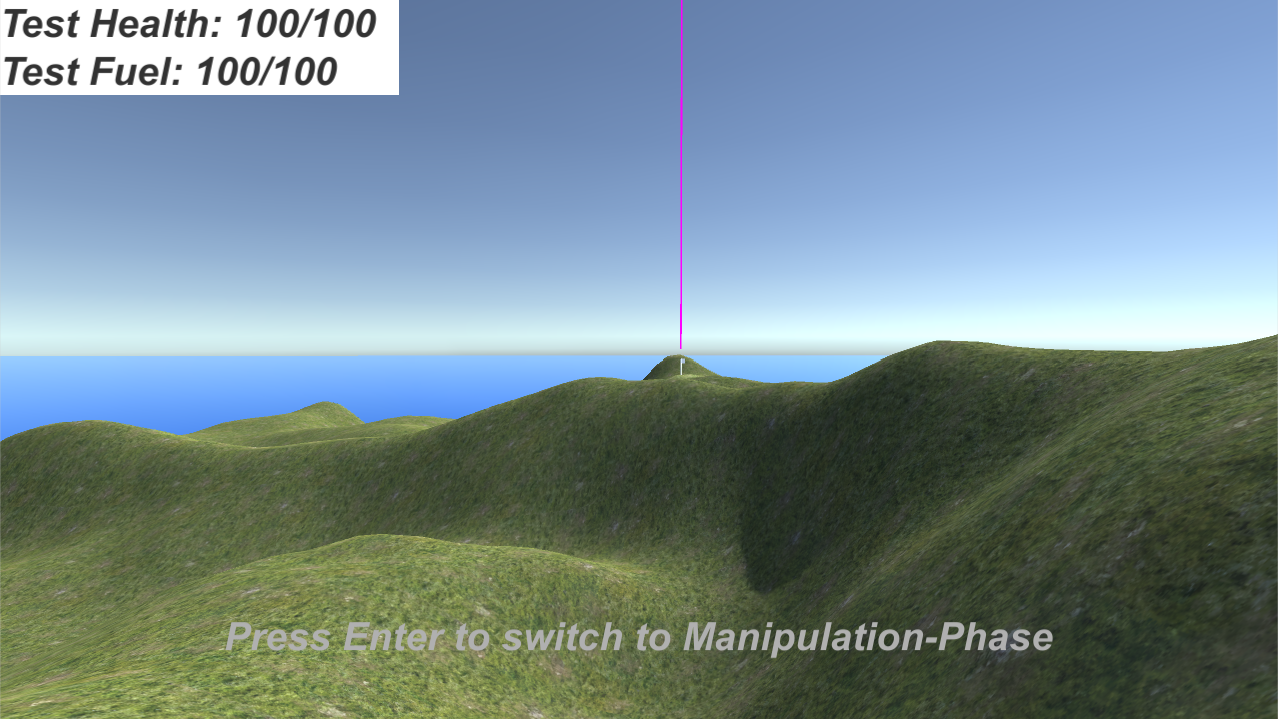
\includegraphics[width=\textwidth]{images/interim/screenshot}
		\caption{Ingame screenshot with UI from Functional Minimum}
		\label{fig:screenshot}
	\end{figure}
	
	\subsubsection{Character Movement}
	Our target for the Functional Minimum was implementing the slide and jet-pack mechanics. The CharacterMovement script handles gravity, velocity slope interactions and is open for other external forces. The Jetpack script receives state messages from the Character script. As long as enough fuel is available and the script is in an "on" state the CharacterMovement script receives an upward motion. Since the basic character and the character movement implementation was split between two different persons, we used multiple interfaces in order to render a smooth development phase possible.
	The CharacterMovement script contains already important parts for the interaction with different terrains planned for the Desirable Target.
	
	\subsubsection{Terrain Manipulation}
	The goal of the manipulation phase was that the player can manipulate the terrain in a way that he/she can raise or lower the terrain at a certain predetermined degree. The player can manipulate the terrain only in the manipulation phase and raises the terrain with a left click, and lowers it with a right click. The manipulation is still not as smooth as it should be and can result in a steeper hill than we would like. But the parameters for the intensity of the manipulation will still need to be checked and adjusted to achieve a balanced gameplay experience. The camera movement was quick and easy to implement. The option to regain charges if the player lowers an already heightened area, is more work than expected and has still to be implemented. An interesting discovery was, that unity saves the changes in the terrain instantly and permanently. To prevent this we must store the unmodified terrain and then use it to reset the terrain after a level is completed or aborted to its original state.
	
	
	\subsection{Low Target}
	Having finished the core mechanics of our game in the Functional Minimum milestone, the focus of the Low Target milestone was making our game actually playable by designing the first level (in this case even the first few levels) and implementing some important gameplay elements like the first turret. Even though the plan was to implement further features regarding the terrain (marking areas as not manipulatable, different surfaces), we did not have enough time for them due to the fact that the implementation of the manipulation itself took longer than expected.
	
	\subsubsection{Level Design}
	The process of designing our first level was iterative and consisted of multiple steps. First we discussed on how and when all our gameplay mechanics should be introduced to the player. We decided that the first two levels are meant as tutorials, where the first only contained sliding and jetpack use and the second one introduced the terrain manipulation in combination with the movement learned before. The next step was that each of our team members designed a level and we voted on the best ones. After that we made minor changes to the selected levels and integrated them into our game.
	
	\subsubsection{Homing Rocket (Turret)}
	The initial design for the homing rocket envisaged a projectile flying at a certain distance over the ground following the player till either a self-destruction timer triggers or its target. However, always keeping distance to the terrain proved to be more difficult than anticipated. Because of a lack of time the rocket design transformed to a simpler design: It just follows the player and explodes when it collides with the ground.
	Since rockets are triggered whenever the player is too close to a turret, an initial velocity ramp up phase is implemented. This prevents a frustrating experience for the player where has no time to dodge the head-on incoming rocket. The acceleration curve is easily adjusted since it is based on Unity's in-built AnimationCurve.
	
	\subsection{Desirable Target}
	
	\subsubsection{Modeling and Arts}
	We are now in the Low Target. The models are needed for the desirable target but I started with them now. 
	
	For modeling I use Blender. I started with modeling two different defense towers. As a reference image I used a typical turbolaser tower from Star Wars.
	One has dual laser guns shooting two lasers at the same time. The other has got one gun shooting rockets. The are suppose to follow the character later on where the dual lasers are shot straight to an old position of the character. With old I mean a few milliseconds after the new position since the character is moving all the time. But the dual laser tower shoots lasers every third seconds so the character has got a chance to avoid a blow. The rockets are shot every 5 or 10 seconds.
	
	The tower, the head (with the wheels) and the guns are all separated meshes.
	
	The lasers are simple stretched capsules also made with Blender like the rockets.
	
	\begin{figure}[H]
		\centering
		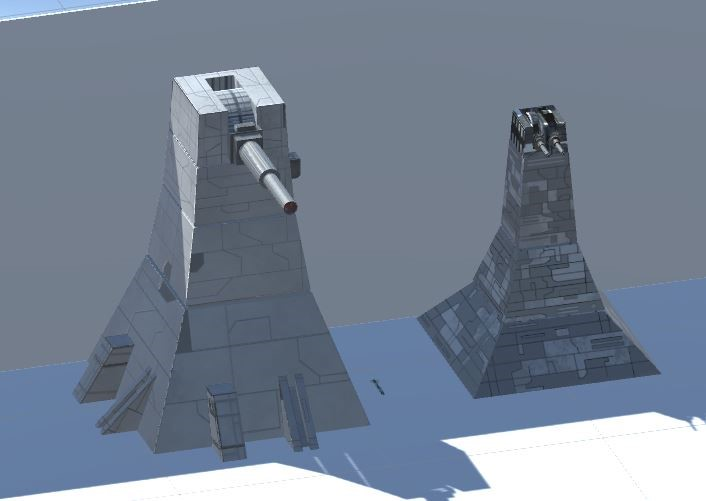
\includegraphics[scale=0.6]{images//interim/turrets}
		\caption{Rocket- and Laser-turret models}
	\end{figure}
	
	\begin{figure}[H]
		\centering
		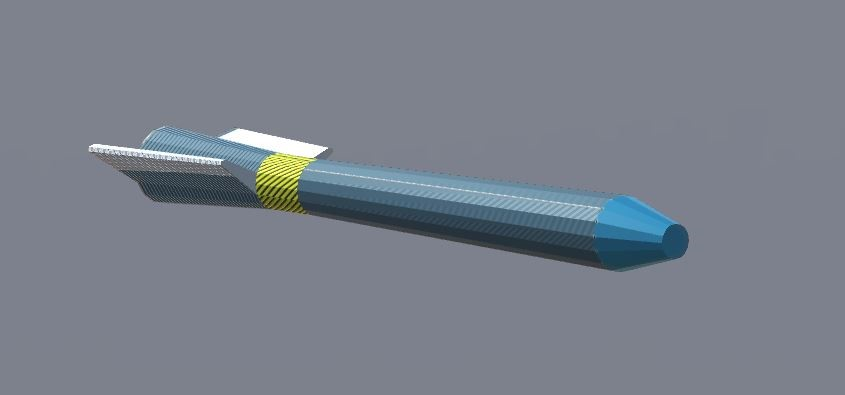
\includegraphics[scale=0.5]{images//interim/rocket}
		\caption{Rocket model}
	\end{figure}
	
	During the cooldown the head of the towers aim the character by moving their heads around the z-axis. At the same time the guns aiming the character rotate planar around the x to y-axis. The guns are attached to the heads. Once the guns shoot they undergo a kickback. The rotations are calculated via scripting using C\# in Unity. The kickback is a simple animation also done in Unity where the gun just go a bit backwards within a very short amount of time to make the kickback fast and then go more slowly to the initial position within a longer amount of time. This is still in process.
	
	The most difficult part is to let the gun rotate around the x and y-axis correctly. The guns are children of the heads so the rotate along the z-axis correctly. But the guns are also attached to a gameObject that is used as a reference point. This game object is placed somewhere under the gun. And if it rotates, the guns rotate around the gameObject to let the player think the gun move along the wheels. Correct setting up this game object as a parent and scripting this special behavior takes the most time.
	
	The textures were made with Gimp where I imported the UV-layout of the guns and drew some lines and dirt effects onto the texture patches. Having done that I created a heightmap and a normal map also with Gimp. These textures are put on the standard shader that is provided by Unity and then applied onto the towers.
	
	Then I modeled the character. I started with helmet and went down to the hands and feet. As a reference image I used a stormtrooper from Star Wars. Then I modeled the jetpack that will be attached to the character as a separate mesh. The visor is a separate mesh too since the material of it will get a glowing effect in the future.
	
	\begin{figure}[H]
		\centering
		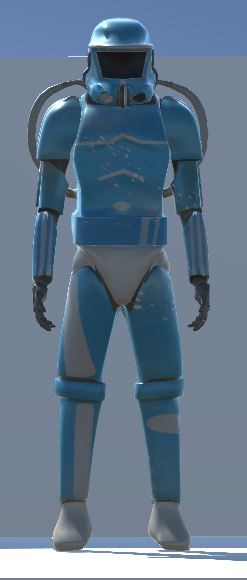
\includegraphics[scale=0.9]{images//interim/character}
		\caption{Character model}
	\end{figure}
	
	The first version of the mesh had more than 50000 triangle. I used the decimated modifier that is provided in Blender to get around 13000 triangles in total. Having a high poly version in the first place makes it easier to model the character.
	It was the first time for me to create a texture of characters. I used to use the "Smart Projecting"-function to unfold a mesh. For this function one does not need to mark seams so it is good for towers for example. At least it is easier for me. But one won't get around of marking seams when texturing a mesh like character. I went through some tutorials and then could create a good UV-layout. I painted it with Gimp then.
	
	In Unity I used again the standard shader with no further special effects to render the textures.
	
	The next new and still a bit difficult part is the animation of the character. I do this also for the first time. I animated all states the character can enter in Blender. Then I imported it in Unity.
	First I got the issue that the each bodypart moved alone without having an effect on the adjacent body parts. This caused the mesh to stretch its neighbors and it looked really bad. This is still in process.
	
	\subsection{Additional Project}
	This section contains a project that can not be classified into one of the layers since it reaches across multiples because of its scope.
	
	\subsubsection{Terrain River}
	The real time river simulation is only dependent on the heightmap of the terrain. It creates rivers by following the path of least resistance till it hits a local minima. Lakes, on the other hand, are created through the filling of a sink. These two phases alternate until a certain min height is reached ($\equalhat$ sea level). 
	The original idea for the path of the river included calculating the current velocity of the stream.  However, this increased the complexity of the algorithm by a large margin and was therefore scrapped. 
	Figure \ref{fig:river1} shows the result of a simulation. In Figure \ref{fig:river2} the player created a dam and rerouted the path of the river.
	
	\begin{figure}[H]
		\centering
		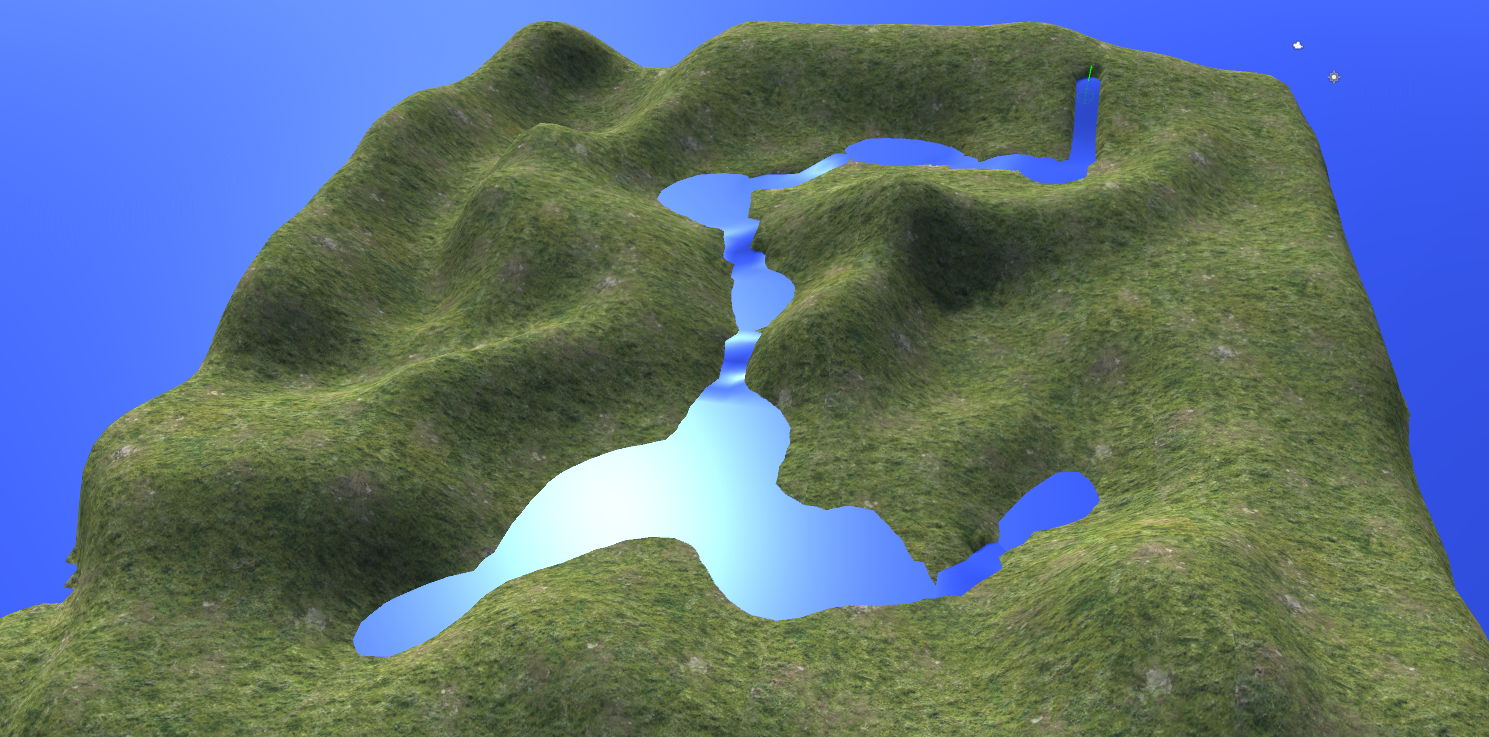
\includegraphics[width=\textwidth]{images//interim/river1}
		\caption{Terrain river without manipulation}
		\label{fig:river1}
	\end{figure}
	
	\begin{figure}[H]
		\centering
		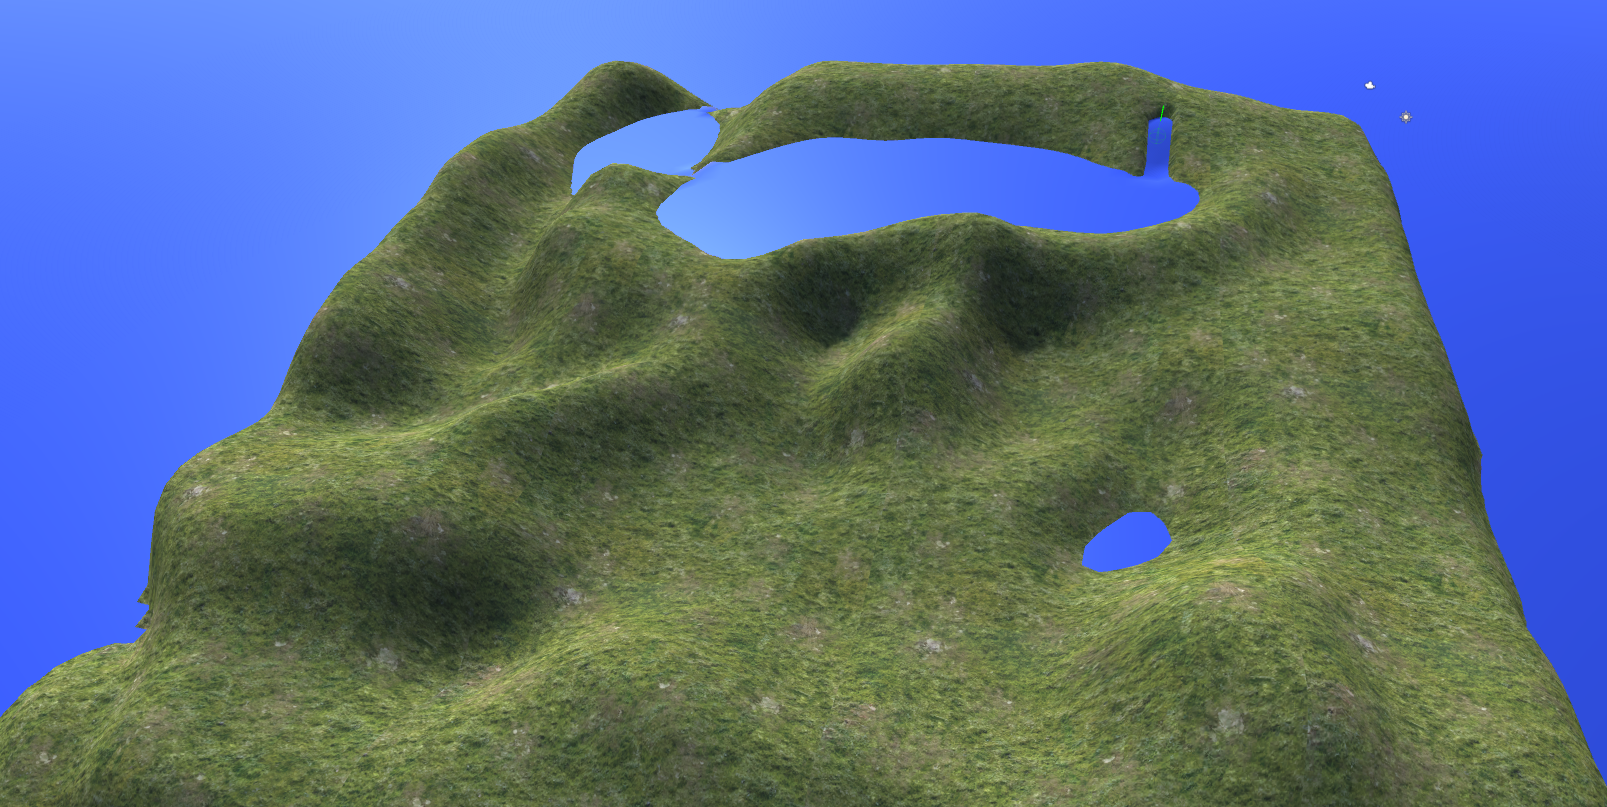
\includegraphics[width=\textwidth]{images//interim/river2}
		\caption{Terrain river with manipulation}
		\label{fig:river2}
	\end{figure}
	
	\newpage
	\section{Alpha Report}
	\subsection{Modeling and Animation}
	I made two new models. A drone and a key. The drone is supposed to be used during the manipulation phase. It can rotate its rotor blades (as one mesh) by having one bone attached to it. The animation is done in Blender goes over 5 frames. The two rotor blades are basically doing two 180 degree rotations around the z-axis. So the there are two keyframes: One is set at 1 and the last at 5 frames.
	\begin{figure}[H]
		\centering
		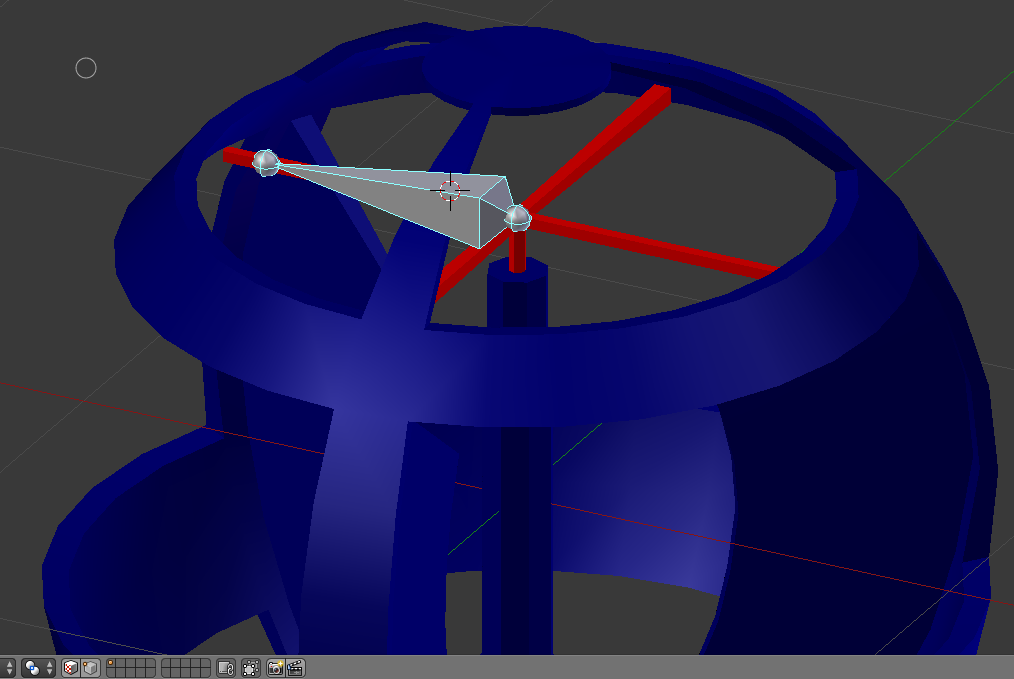
\includegraphics[scale=.3]{images//alpha/droneBone}
		\caption{Bone of drone propeller}
	\end{figure}
	No script is used for the animation. Since Unity needs a root bone what was new to me I had to add one to get it work.
	\begin{figure}[H]
		\centering
		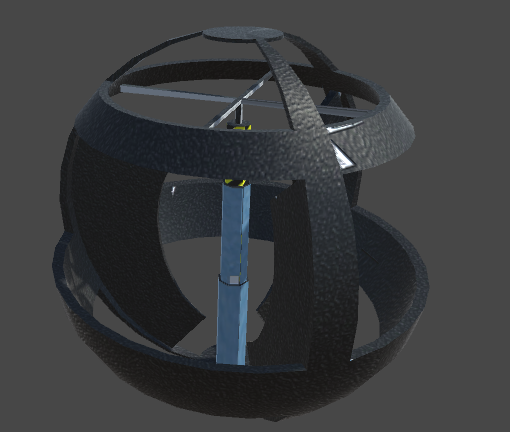
\includegraphics[scale=.6]{images//alpha/drone}
		\caption{Textured drone}
	\end{figure}
	A further model is the key that the player will need to open certain doors. The texture and the normalmap were done in Gimp.
	\begin{figure}[H]
		\centering
		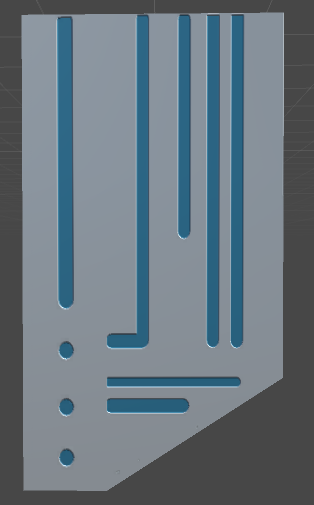
\includegraphics[scale=.4]{images//alpha/keycardModel}
		\caption{Keycard}
	\end{figure}
	The animation of the character is also done completely in Blender. An amature sticks to the mesh. Certain mesh parts are weight painted so that the correct mesh part refers to the correct bone when moving.
	\begin{figure}[H]
		\centering
		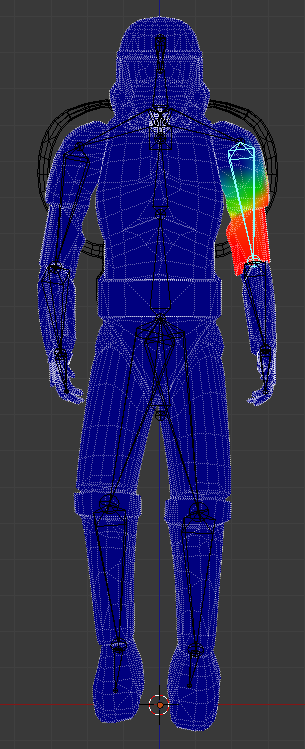
\includegraphics[scale=.5]{images//alpha/boneWeights}
		\caption{Bone weights}
	\end{figure}
	So in this case the bone of the left arm let the left arm of the mesh move smoothly.
	
	First the mesh itself was too big for the scene in Unity. Scaling it down along with the armature caused suddenly some issues with the uv-coordinates. The texture coordinates of the mesh were reset for some reason and I had to reassign them again. Due to the "transfer uv-map"-function it was possible to transfer the correct uv-map that was assigned to an old model to the new animated model with the wrong uv-coordinates.
	
	The different poses that the model can enter are all done in one whole animation frame. The poses are states, representing: flying forward, neutral, flying backwards, flying sidewards, falling, flying upwards.
	\begin{figure}[H]
		\centering
		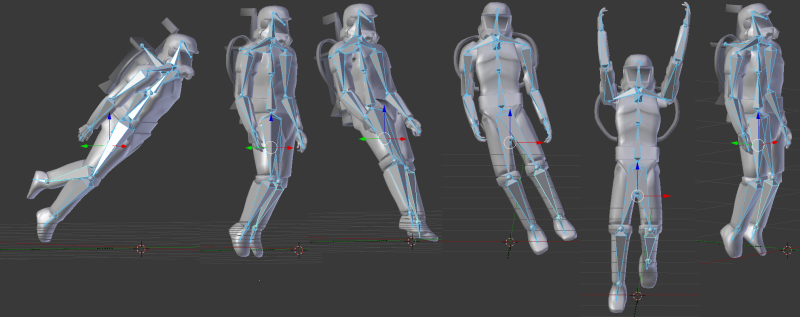
\includegraphics[scale=.7]{images//alpha/allAnimations}
		\caption{All postures}
	\end{figure}
	The respective frames will be accessed via script.
	
	\subsection{Particle Effects}
	As a desirable target particle effects were added to game. They were created with the help of the built-in particle system of Unity. Figure \ref{fig:rocketTrail} shows the propulsion fire and a smoke trail that is left behind for a few seconds. The rocket explodes either after a time limit is reach or as soon as it comes in contact with object (Figure \ref{fig:explosion}). 
	
	If the player manages to win a level a firework particle system is spawned (Figure \ref{fig:fireworks}). The specific characteristic of the latter is that a shot particle spawns an additional particle system upon death. 
	\begin{figure}[H]
		\centering
		\begin{tabular}{ccc}
			\subfloat[Rocket trail fire FX]{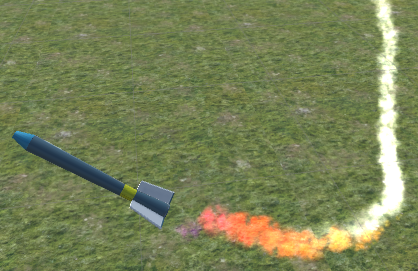
\includegraphics[scale=0.5]{images/alpha/RocketTrailFireFX}\label{fig:rocketTrail}}&
			\subfloat[Explosion FX]{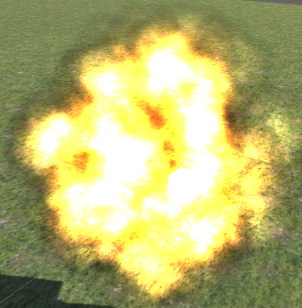
\includegraphics[scale=0.5]{images/alpha/ExplosionFX}\label{fig:explosion}}&
			\subfloat[Fireworks FX]{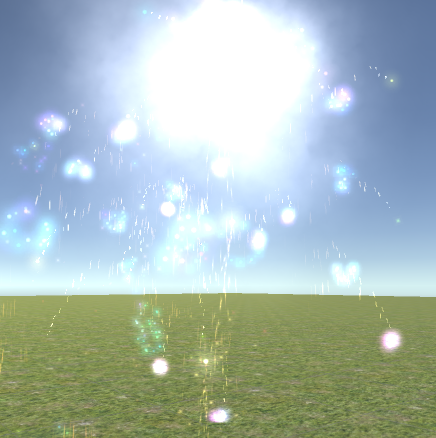
\includegraphics[scale=0.5]{images/alpha/FireworksFX}\label{fig:fireworks}}
		\end{tabular}
		\caption{Second Level}
	\end{figure}
	
	\subsection{User Interface}
	Another important part of our desirable target was a proper UI. This includes both a nice main menu, as well as a fancy display of ingame information like fuel and health.
	
	 The concept of the main menu was to have a 3D scene with all available levels arranged around the camera, which is freely controllable by the player. This is a nice way to display the variety of different terrains and our player models. Furthermore the are basic buttons like \textit{Options} and \textit{Exit}. A first draft of the main menu can be seen in Figure \ref{fig:mainMenu}.
	 \begin{figure}[H]
	 	\centering
	 	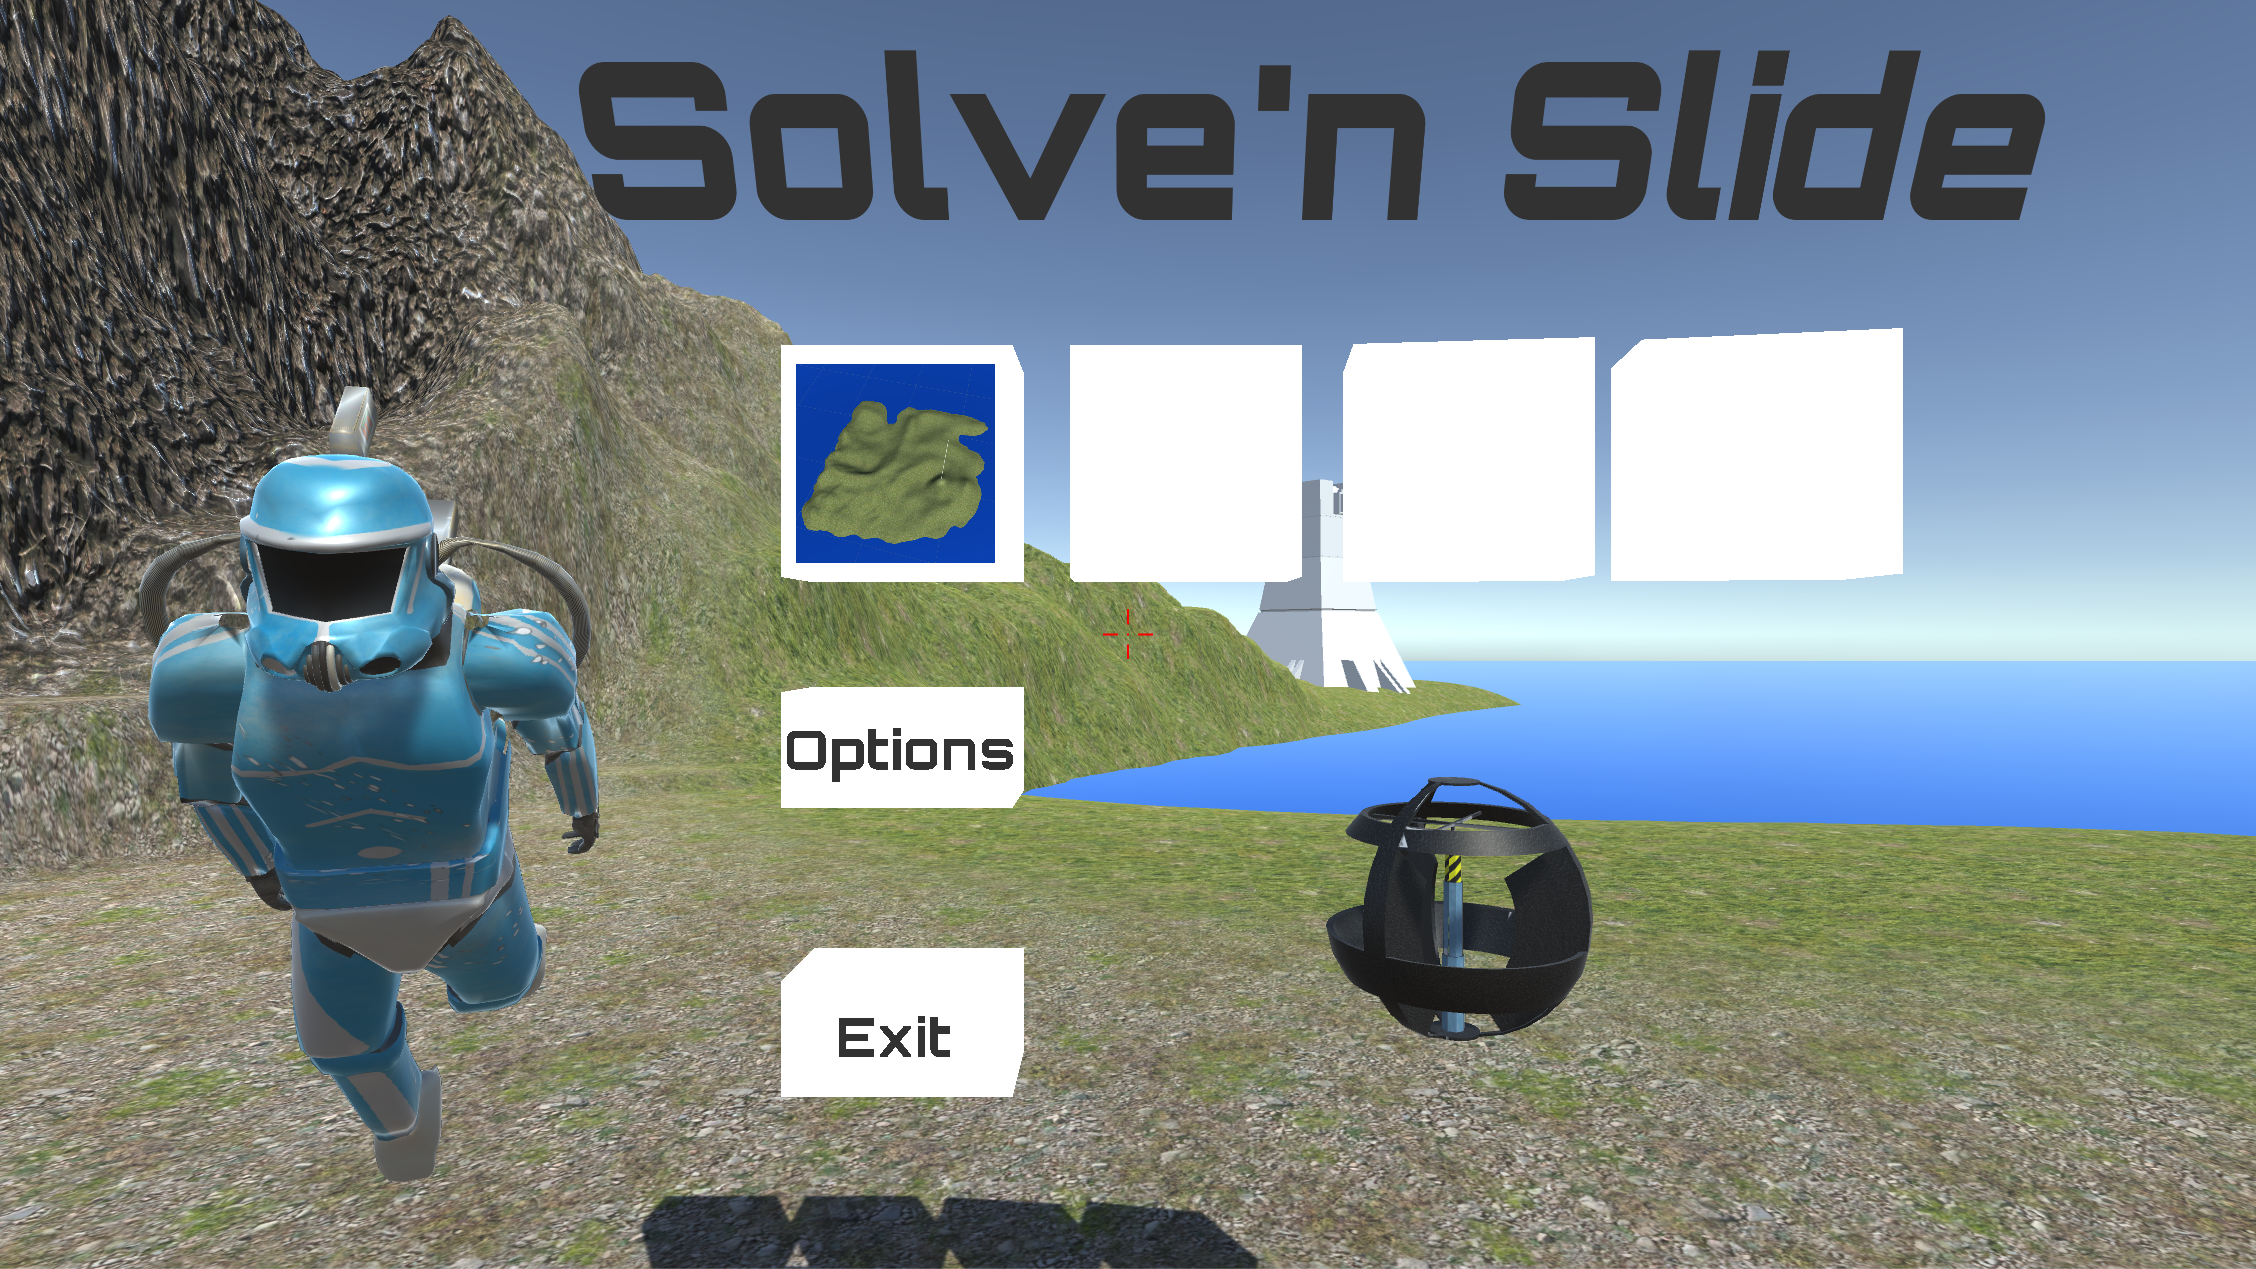
\includegraphics[scale=.17]{images//alpha/mainMenu}
	 	\caption{First draft of main menu}
	 	\label{fig:mainMenu}
	 \end{figure}
	 
	 For our ingame UI we needed three different icons representing the number of terrain manipulation charges, the amount of placeable fueltanks and the collected keys. These can be seen in Figure \ref{fig:icons}. The charge and fueltank icons turn black and white once the player used one of them.
	 \begin{figure}[H]
	 	\centering
	 	\begin{tabular}{ccc}
	 		\subfloat[Charge icon]{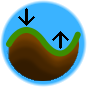
\includegraphics[]{images/alpha/chargeIcon}\label{fig:chargeIcon}}&
	 		\subfloat[Fueltank icon]{
\includegraphics[]{images/alpha/fuelTankIcon}\label{fig:fuelTankIcon}}&
	 		\subfloat[Key icon]{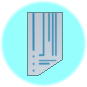
\includegraphics[]{images/alpha/keyIcon}\label{fig:keyIcon}}
	 	\end{tabular}
	 	\caption{Ingame UI icons}
	 	\label{fig:icons}
	 \end{figure}
	 
	 The last part of the ingame UI is to display fuel- and healthbars. These can be seen in Figure \ref{fig:fuelAndHealth}. In Unity the obvious solution for these would be to have filled sprites, but the problem with this method is the vertical edge, which looks wrong for this layout. Instead the individual bars were moved left and right and then masked to only show the visible are and prevent them from overlapping.
	 \begin{figure}[H]
	 	\centering
	 	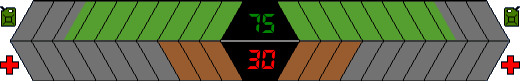
\includegraphics[scale=.8]{images//alpha/fuelHealthBar}
	 	\caption{Fuel- and healthbars}
	 	\label{fig:fuelAndHealth}
	 \end{figure}
	 \subsection{Terrain Manipulation}
	 \subsubsection{Better Terrain Manipulation}
	 The terrain manipulation was improved by a better formula. Instead of increasing the terrain like a pyramid, the terrain calculates the change like a half sphere and adds it to the terrain. There is also now a highlighted area with which the player can better determine how much he/she is going to change.
	 
	 \subsubsection{Regain Charges (Undo Option)}
	 To enable an undo option in this type of game, we had to place a marker with the exact position of the change. If the marker is clicked with the opposite terrain modification then the terrain is changed back and one charge is regained. 
	 
	 If the player switches from the manipulation phase to the action phase or vice versa. The markers need to be deactivated or reactivated. In order to do this, the markers are stored in an updated list, from which all markers are accessible. 
	 
	 \subsubsection{Unmodifiable Terrain}
	 In order to determine which terrain is modifiable and to make it easy for the developers to create a level, we added unmodifiable textures for each used texture we have. Areas that can't be modified in the manipulation phase are shown with a reddish color. If a player tries to change a piece of terrain, the algorithm checks which texture is hit and if it is one of the unmodifiable terrains then nothing will happen. As the player switches to the action phase the unmodifiable textures are replaced by their respective "normal" textures, for aesthetic reasons. 
	 
	 \subsubsection{Terrain Characteristics}
	 Different terrain textures have different friction which influences the speed of the player. If the player is touching the terrain, it will be determined on which texture the player stands and the appropriate friction will be used for the speed calculation of the player.
	 
	 \subsection{Miscellaneous}
	 \subsubsection{Fuel Tanks}
	 The player can now place fuel tanks, for him to pick up in the action phase. Fuel tanks can be placed in the manipulation phase, which now has two modes. In the first mode the player can manipulate the terrain and in the second he/she can place the fuel tanks. Fuel tanks can be placed anywhere in the map, they are placed a few meters in front of the player.
	 
	 \subsubsection{Doors and Keys}
	 In the game there are now levels, which use keys and doors. Keys and doors are already placed by the developer and can't be moved by the player in the manipulation phase. The player has to pick up the keys in the action phase in order to open the doors, which are represented as a forcefield and block important areas like the path to the goal.
	 
	 \subsubsection{Sound Effects}
	 Sound effects were added to the game, which are realized by a musicbox object in the game. For the wind sound effect we used a script to determine how fast the player is, to adjust the volume of the sound effect, with which the player gets a better feeling how fast he currently is. 
	 
	 \section{Playtesting}
	 After our successful alpha release we temporarily froze the development of our game to build a standalone version of the current status that all of our team members used for playtesting. To summarize the most important aspect of playtesting, which is how much fun the game was, the survey resulted in a solid 3.9/5 for fun and a 4.3/5 for the concept.
	 \begin{figure}[H]
	 	\centering
	 	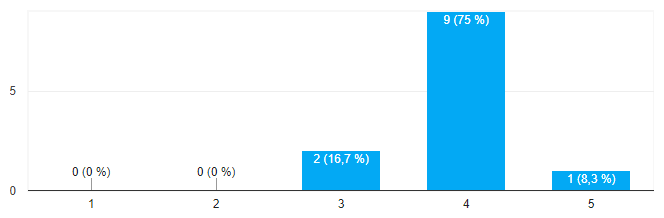
\includegraphics[width=\textwidth]{images/playtesting/fun}
	 	\caption{How much fun was the game?}
	 	\label{fig:fun}
	 \end{figure}
	 \begin{figure}[H]
	 	\centering
	 	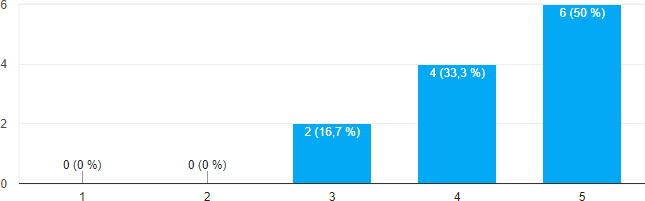
\includegraphics[width=\textwidth]{images/playtesting/concept}
	 	\caption{How did you like the concept? }
	 	\label{fig:concept}
	 \end{figure}
	 
	 \subsection{Testing procedure}
	 The first goal of our playtesting phase was to find good questions to ask our testers after they played our game. Once we had a good selection of varying questions we created a Google Forms survey which our testers could fill out after playing. In the next step all team members approached friends and families to ask them to participate in the tests. These were conducted in three different ways. 
	 
	 The first and best one was to be with the tester in one room in front of a computer running the game (7 times). The advantage of this approach was that we could see exactly what the tester was doing, what his reactions were and if he had trouble with the controls. Furthermore we could, in case of bigger troubles, demonstrate how things work, which gladly only occurred with parents that never played a computer game in their life. The second way was to use Skype with screen sharing (6 times). This still enabled us to see what the tester is doing ingame, however we had to rely on comments from him to determine his emotions and problems. The last way also used Skype but with screen sharing turned off. With this approach we had to completely rely on comments from the testers, which is why we tried to avoid using it (2 times).
	 
	 Overall we had 15 participants with 12 of them completing our survey. There were 10 males and only two females, ranging in age from 16 to 27 (see Figure \ref{fig:ageDistribution}) of which all of them considered themselves as relatively good gamers. Even though the survey contains 25 questions we will only cover the ones with an interesting and meaningful result in the following sections. 
	 
	 \begin{figure}[H]
	 	\centering
	 	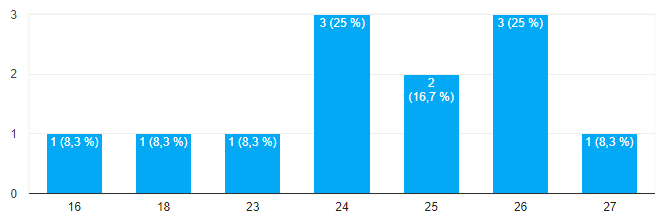
\includegraphics[width=\textwidth]{images/playtesting/ageDistribution}
	 	\caption{Age distribution}
	 	\label{fig:ageDistribution}
	 \end{figure}
	 
	 \subsection{Graphics}
	 The first part of the game that the player gets to see, the main menu, was one of the most controversial topics of the survey, with at least one vote for each of the five options ranging from \textit{"Did not like at all"} to \textit{"Liked it a lot"}. However on average people tended to rather like it than dislike it with an rating of 3.3/5. The reasons for disliking it were mostly that the level preview images looked strange and that the options button did not work. The strange looking images have already been fixed and the options button will be removed since Unity offers these in the launcher by default.
	 
	 The next graphical aspect was the user interface. On average it got a rating of 3.5/5 with the biggest complaint being a inconsistent display of the fuel amount, meaning that a full bar is showing the maximum per level and not a global maximum with different starting amounts per level. Hopefully this won't be a problem once players are more familiar with the game and automatically check the displayed number in the fuel bar UI. Another complaint was not knowing how much fuel you have in the manipulation phase, which resulted in changing to the action phase just to see the amount of available fuel.
	 
	 Another aspect regarding graphics were the 3D models. They were generally liked, with only one person mentioning that the manipulation character model does not look like a drone or camera. 
	 
	 The most disliked thing about the graphics was the environment. The levels looked empty, so we plan to implement grass and trees and the water and forcefields were not really recognized as what they should be which we will fix by introducing some animated textures and shaders.
	 
	 \subsection{Controls}
	 For people familiar with computer games controlled by keyboard and mouse the inputs for the action phase were very intuitive. Only complaints were that the movement on the ground was too sluggish and there wasn't enough control, so we might have to rethink the way our movement works. One tester wished there was a way to restart the action phase with one button press (e.g. 'R') instead of switching to the manipulation phase and back again, which can be easily implemented.
	 
	 Since some information regarding key bindings for the manipulation phase were not mentioned in the info text, we had to explain some of them to our testers. Once they knew all the bindings, the control for the manipulation phase was quite clear for them. They were not as intuitive as the ones in the action phase, but they were still manageable. Some people would prefer to control the height of the character either with a combination of shift/ctrl/space or by moving in the direction you are looking at. Furthermore most testers had troubles undoing terrain manipulations or placed fuel tanks so there is the need of fine tuning, which already happened to a certain degree.
	 
	 \subsection{Gameplay}
	 There were some issues that occurred during the game.
	 One is that the main part of scripting was done within the Update function instead of FixedUpdate. So it happed on very fast computers that the character or the camera moved too fast due to high fps.
	 Before starting the actual game one has the choice between several screen resolutions and graphics qualities. It happened sometimes that the game crashed when having selected the fastest setting or even in the opposite case when the game crashed on anything but "fantastic".
	 The drone's height-value is constant but some mountains are higher and so the drone just flies through the mountain without letting the player look at that mountain. It can also happen that some fuel tanks can land under the terrain or outside map when placing them.
	 An obvious bug is the fact that one can bury the character during the manipulation phase. When switching to the action phase the character falls through the ground. The goal can be buried aswell and thus the level is not completable. Some thought it is a bug that one can bury the turrets too but it can also be seen as a possibility to reach the goal in this certain way. When the turret is buried the rockets can not go fly through. When pressing "2" to place a fuel tank the fuel tank appears every time when starting a level until the player presses "1".
	 
	 \subsection{Leveldesign}
	 \textbf{First level:}
	 The manipulation phase was too short since one couldn't really do anything. The player is some kind of cursed with dissipation of time by having tried a lot of different buttons (except of enter to switch the phase) without getting any further. This level also felt a bit "lonely" due to a lack of decoration, for example missing trees. Since the first level is a tutorial there should be definitely be the hint that says to press enter to switch the phase.
	 Then entering the action phase the player was a bit surprised that he is suddenly starting to fly around. Some also got reminded of the game Tribes.
	 The character's initial position is too deep into the ground. So to start moving the player had to press the moving button a while. This loaded the momentum really high and gave the character all of a sudden really high velocities.
	 At the end the players were able to complete the level successfully. Some didn't like the design of the goal marker.
	 
	 \textbf{Second Level:}
	 Some players had some problems with the second level and also said it was the hardest level, which needs to be adjusted since it is also a tutorial level.
	 
	 \textbf{Third Level:}
	 The idea of the key design was to design some kind of a futuristic key. But it wasn't recognized as this and the players got confused. They thought it is a chip or even a mini drawn map. At the first glance some even considered the key to be the goal.
	 We planned that one has to collect the key and then be able to fly through the blue wall in order to reach the goal. But after flying randomly along the map the players got to the goal without having collected the key.
	 Most players were a bit overwhelmed. They felt left alone with the whole terrain. The blue wall was a mystery, icons were too. When flying they didn't realize that they are out of fuel.
	 
	 \textbf{Fourth Level:}
	 Because of the bug that on fast computers the character moved too fast, this level was solved too easily and on slow computers this level was way harder than it was intended.
	 
	 \textbf{Fifth Level:}
	 Some wished the level to have better light effects light better ambient lighting.
	 
	 \textbf{All in all:}
	 In each level the amount of jetpacks is different. Some thought that this was a bug. But we did it on purpose as we wanted to adjust the balancing. The player liked that there were different ways to reach the goal in each level. But still each level was too easy to solve.
	 
	 \subsection{Balancing}
	 The overall average balancing and difficulty of the game is alright, but it still needs a lot of work, because it has a wide range of different opinions. Like some levels are too easy and some are too hard. We need to work on these to get to a better average result of opinions.
	 We also still have a lot of inconsistency in our levels, like different amounts of fuel in the jetpack, different settings for the turrets, etc. which need to be equated or to be shown properly to the player so that he has a better understanding for the map.
	 Another important issue was the fact that the collision box of the fuel tanks and the keys were not really big enough. That is because the player doesn't have an absolute control where he is sliding/flying and often just flies a few meters by the fuel tank / key. Which is why the collision box needs to be much bigger than the mesh object itself.
	 Our goal for balancing will be, that the player has a good time and the game will not be too hard, but still has enough challenges so that he/she still has to think about the problems and doesn't get bored too easily.
	 
	 \subsection{Sound effects}
	 As seen in Figure \ref{fig:sound}, the testers were not impressed by the sound effects, but still think that overall it was alright, and was also clear which sound was produced by which action.
	 
	 \begin{figure}[H]
	 	\centering
	 	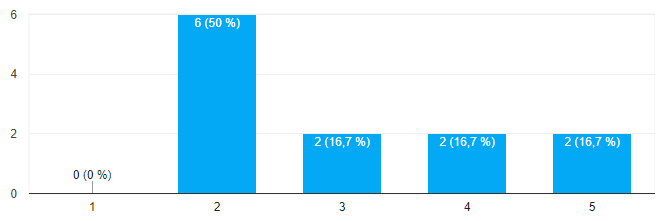
\includegraphics[width=\textwidth]{images/playtesting/sound}
	 	\caption{How did you like the sound effects?}
	 	\label{fig:sound}
	 \end{figure}
	 
	 The key issues, which need to be fixed, were the following: The sound effects were in some cases too loud, like when the player places the fuel tank in the manipulation phase. There were no sound effects when the turrets shot, when the rockets exploded or when the fuel tank was picked up. And also in enough cases the wind sound was mistaken for the jetpack sound, because the jetpack sound was not playing, and also because the wind sound is not clear enough for some speakers.
	 
	 \subsection{Wishes and Suggestions}
	 We got a lot of different wishes and suggestion in which way we could improve our game. Most of them were for the improvement of the visual/graphical look of the game, to make the game more intuitive/understandable for the player and to add more options for the player and level designer to use so that the game will become more complex.
	 \bigbreak
	 The most wished changes were the following:
	 \begin{itemize}
	 \item Different difficulties for the game, so that the players don't have a boring or frustrating experience.	
	 \item A proper tutorial or at least texts with complete explanation what is possible in the game and what the player needs to be aware of.
	 \item More manipulation options, like the form in which the terrain is changing, or the gadgets you can place around the map.
	 \item Sound effects which were missing in some cases, as explained in section "Sound effects”.
	 \item To have an option/mode with which you can place the fuel tank always on the point of the ground which the player is looking.
	 \end{itemize}
	 
	 \newpage
	 \section{Final Release}
	 \subsection{Changes}
	 \subsubsection{Force Field}
	 Our idea of a key/lock system was realized with a key card and a force field. However, latter was originally only a transparent box. Therefore we implemented force field shader, that changes over time (Figure \ref{fig:forceField}). Additionally, we introduced a color coding system for the keys and locks which allowed to created more complex levels. The color change of the keys was realized with the help of a rim shaded sphere that also helps visualizing the extent of the collider.
	 \begin{figure}[H]
	 	\centering
	 	\includegraphics[width=\textwidth]{images/final/ForceField}
	 	\caption{Animated, colored force fields and keys (inc. GUI)}
	 	\label{fig:forceField}
	 \end{figure}
	 
	\subsubsection{Environment}
	As already mentioned a large point of criticism was the empty-looking environment. We started with improving the sky. With the help of a particle system we archived a reasonable looking clouds which move over time (Figure \ref{fig:movingClouds}). Moving cloud shadows are faked with the help of unity's so-called “light cookie” (Figure \ref{fig:movingShadows}).  We also made use of Unity's lens flare.
	\begin{figure}[H]
		\centering
		\begin{tabular}{cc}
			\subfloat[Timestep 0]{\includegraphics[scale=0.33]{images/final/MovingClouds1}}&
			\subfloat[Timestep 1]{\includegraphics[scale=0.33]{images/final/MovingClouds2}}
		\end{tabular}
		\caption{Moving clouds}
		\label{fig:movingClouds}
	\end{figure}
	
	\begin{figure}[H]
		\centering
		\begin{tabular}{cc}
			\subfloat[Timestep 0]{\includegraphics[scale=0.33]{images/final/MovingCloudsShadow1}}&
			\subfloat[Timestep 1]{\includegraphics[scale=0.33]{images/final/MovingCloudsShadow2}}
		\end{tabular}
		\caption{Moving cloud shadows}
		\label{fig:movingShadows}
	\end{figure}
	
	Another point of improvement was our level boundary: the water plane. First of all, we exchanged the plain opaque shader with a refractive shader provided by Unity. Additionally, we created an editor script that enabled us to created a smooth transition between the terrain and the ocean floor, which is a black plane (Figure \ref{fig:water}). 
	\begin{figure}[H]
		\centering
		\includegraphics[width=\textwidth]{images/final/Water}
		\caption{Refractive water and underwater transition}
		\label{fig:water}
	\end{figure}
	
	\subsubsection{Menus}
	In order to give our game a more fun, cartoonish look we made the title of our game inside the main menu an overhaul (Figure \ref{fig:title}). First of all it is now written with 3D font. Secondly, the color of every letter changes every time the game is start up. However, they are always saturated. Finally, the letters bounce up and down for a while (Figure \ref{fig:title}).
	\begin{figure}[H]
		\centering
		\begin{tabular}{cc}
			\subfloat[Timestep 0]{\includegraphics[scale=0.4]{images/final/Title1}}&
			\subfloat[Timestep 1]{\includegraphics[scale=0.4]{images/final/Title2}}
		\end{tabular}
		\caption{Title at startup}
		\label{fig:title}
	\end{figure}
	
	Besides a general look overhaul for the main menu (Figure \ref{fig:mainMenuFinal}) we exchanged the non-functional options button for a credits button and implemented it (Figure \ref{fig:credits}). You can close the window with by pressing any button.
	\begin{figure}[H]
		\centering
		\includegraphics[width=\textwidth-1cm]{images/final/MainMenu1}
		\caption{Partial main menu screenshot}
		\label{fig:mainMenuFinal}
	\end{figure}
	\begin{figure}[H]
		\centering
		\includegraphics[width=\textwidth-1cm]{images/final/Credits}
		\caption{Credits screen}
		\label{fig:credits}
	\end{figure}
	We added a menu and a pause functionality during both phases.
	\begin{figure}[H]
		\centering
		\includegraphics[]{images/final/PauseMenu}
		\caption{Pause menu}
		\label{fig:pauseMenu}
	\end{figure}
	
	\subsubsection{Drone}
	Since most testers did not realize at first that you are controlling a drone during the manipulation phase we decided to change things up a bit. First of all, we changed the default camera look rotation to downwards and limited the rotation upwards. Next, we increased the field of view which strongly improved the feeling of looking through a drone camera. With the help of Unity's Post Processing Stack we added a lot of camera effects: Saturation increase (through the color grading system: Academy Color Encoding System), bloom, motion blur, depth of field and anti-aliasing. Figure \ref{fig:sceneWithoutEffects} depicts a scene before all of these changes (and without fog) while Figure \ref{fig:sceneWithEffects} shows the same scene afterwards. Finally, we improved the controls.
	\begin{figure}[H]
		\centering
		\includegraphics[width=\textwidth-4cm]{images/final/DroneEffects1}
		\caption{Scene without most effects}
		\label{fig:sceneWithoutEffects}
	\end{figure}
	\begin{figure}[H]
		\centering
		\includegraphics[width=\textwidth-4cm]{images/final/DroneEffects2}
		\caption{Same scene with effects}
		\label{fig:sceneWithEffects}
	\end{figure}
	
	\subsection{Conclusion}
	The experience of the class was good, we learned a lot and it was fun. The game idea did materialize very well and everything till the desirable targets was implemented, but only one high target and one extra were made. The terrain manipulation took in the beginning longer than expected, but then everything else was done according to schedule. Overall the development schedule helped a lot because we had to think beforehand what needs to be done, and because of that we could distribute the work much better and we didn't have to think much about what needs to be done, but could instead concentrate much better on the tasks that everyone had. The prototype was not too bad, because we learned early that the level design will be very hard and that we will have to put much thought and work into it. But in our special case it didn't really help us to determine how much fun the manipulation and action phase has to offer and also what kind of settings should be used for the phases. The playtesting session was really good, it helped the most for our development, because we found many bugs and many new ideas were given to us on how we could improve the game. We also discovered that our game was too hard and a more casual and fun oriented approach would be better suited for our game. Overall it would be better if the playtesting phase was much earlier and even more often. But we know that because of how short a semester is, it is not really feasible to change the schedule to have much more playtesting, and we think the schedule is for the amount of time alright as it is.
	
	The course itself was good and it did meet our expectations. We learned quite some things in this class. The schedule was good as it was, it wasn't too much work at once and there was enough time to implement the different stages of the game. And overall we think we did a good job and are happy with the results.
	
	The biggest technical difficulties in our project were the level manipulation and the animations, because it was new to us. But after we learned how to do it, it wasn't that difficult and overall we didn't have much problems.
	
	To have overall a theme is not bad, because it gets you in a direction and you get faster to results. In our case the theme speed, has received mixed feelings, some found it good and were happy with it, some others would like to have total freedom, because it was wished to have more storytelling in the game but it was not really possible with this theme and game idea.
	
	With the experiences that we learned here, we would in our next game project do playtesting much more and often, because you find more bugs and you see much earlier if you are going in a right or wrong direction. We also would sit together much more often and test together on one pc, because we could work better on problems together and also help each other better.
	
	Great successes for us were to learn how to do animations and terrain manipulations properly and overall that all targets till desirable targets were met and we have an overall complete game.
	
	We managed to meet all targets till the desirable target always in time and not one target has been dismissed. But we didn't have much time to do the high and extra target but we still managed to implement one of each.
	
	We think it would be better if the course schedule were changed so that we have to upload our game at each milestone, and that every participant has to play the game of the other groups and to give a comment on that, so that there would be a small playtesting phase between each milestone.
	 
\end{document}